\documentclass[titlepage,dvipdfmx]{jsarticle}
\usepackage[dvipdfmx]{graphicx}
\usepackage{url}
\usepackage[dvipdfmx]{hyperref}
\usepackage{multirow}
\usepackage{pdfpages}
\usepackage{listings, jvlisting}
\usepackage{float}
\usepackage{verbatim}
\usepackage{wrapfig}
\usepackage{dcolumn}
\usepackage{bookmark}
\usepackage{longtable}
\usepackage{color}
\usepackage{ulem}
\usepackage{caption}
\usepackage{subcaption}
\usepackage{amsmath,amssymb}
\usepackage{amsthm}
\usepackage{mathtools}
\usepackage{bm}
\usepackage{proof}
\usepackage{bussproofs}
\renewcommand{\figurename}{図}
\renewcommand{\tablename}{表}
\newcommand{\Add}[1]{\textcolor{red}{#1}}
\newcommand{\Erase}[1]{\textcolor{red}{\sout{\textcolor{black}{#1}}}}
\lstset{
  language={C},
  basicstyle={\small},%標準書体
  identifierstyle={\small},%
  commentstyle={\small\itshape},%
  keywordstyle={\small\bfseries},%
  ndkeywordstyle={\small},%
  stringstyle={\small\ttfamily},
  frame={tb},
  framesep = 5pt,
  breaklines=true,
  columns=[l]{fullflexible},%
  numbers=left,%
  xrightmargin=0zw,%
  xleftmargin=3zw,%
  numberstyle={\scriptsize},%
  stepnumber=1,
  numbersep=1zw,%
  lineskip=-0.5ex,%
  keepspaces=true,
  showstringspaces=false
}
\renewcommand{\lstlistingname}{Code} 
\begin{document}
\title{卒業論文\\シーンマッチングによる自動運転ナビゲーション\\}
\author{\\学籍番号:T190022\\氏名:大野 大樹}

\maketitle
\tableofcontents
\newpage
\section{序論}
\subsection{研究の背景と目的}
\subsubsection{背景}
近年、人工知能の機械学習法の著しい発展により、自動運転や無人ドローンといった自律走行、自律飛行技術への関心が高まっている。
自動運転を搭載した車では、スバルアイサイト\cite{f1}のように周囲の情報をステレオカメラのみを使用したものがあるが、
テスラModel3\cite{f2}やトヨタAdvanced Drive\cite{f3}といった3次元センサー(3DLidar)とステレオカメラを使用して取得しているものもある。
3次元センサーを用いることで、道路の路面状況、車間距離、歩行者の有無といった周囲の状況をより緻密に把握することができ、
光を使わないため暗闇や雨天など天候の影響を受けにくいという特徴を持っている。
しかし、周りに障害物のない開けた土地やデータ処理の負荷が高い、そしてセンサーそのもののが高価であるなどのデメリットもある。
また、カメラセンサーは天候の変化や暗闇に弱いというデメリットはあるが、画像の解像度の向上や画像から得られる情報の多さ、3次元センサーと比べコストが低いというメリットがある。
そこで、本研究では3次元センサーと比べ比較的安価であるカメラと基本的な画像処理を用いた自己位置推定を行っていく。
%しかし、自律走行への技術チャレンジ事態は1977年にIEEE(Institute of Electrical and Electronics Engineers)が提唱したマイクロマウス競技から始まっている。
%マイクロマス競技とは、マイクロマウスと呼ばれる小型自律走行自動運転車両を使用し、迷路の4隅のいずれかのスタートから始まり迷路中央にあるゴールへと到達する時間を競う競技である。
%日本でも1980年に公益財団法人ニューテクノロジー振興財団が主催として今年で42回目を迎える「全日本マイクロマウス大会」がある。
%マイクロマウス競技では主催者によって規格を定められ、人工的に作られた経路の中での自律走行を行うという特徴がある。
%しかし、実世界で自動運転車両が自律走行を行う場合、競技と同じように誰かに規格され自律走行専用に整備された場所で自律走行を行うわけではない。
%我々人間が暮らす空間に自動運転車両が存在するためには、絶えず変化する環境で自律走行を行わなければならい。
%そのためには、そういった環境で実験ができる場所と機会が必要である。
%2007年3月に公道での自律走行自動運転車両実証実験「つくばチャレンジ」が始動した。
%現在のつくばチャレンジでは、つくば市内の遊歩道からなる2kmのコースを本走行前の事前走行等のデータを使用して、本走行では自動運転車両のみの完全自律走行を行う実証実験である。
%我が群馬大学は、学生が主導で研究しているMercury Academic Modelが2018年以来となる本走行での完走を果たした。
\subsubsection{目的}
自動運転車両が目的地まで移動する場合、自動運転車両は現在の位置を知る必要がある。
これを自己位置推定という。例えばLiDARなどのセンサーを用いる場合、
自己位置推定は環境の3Dデータを持つ地図と、現在の環境の形状を3次元的に
照合すること等で自己位置推定を行う。しかし、人間は周囲の風景を見て、自分の位置を
知ることができるため、自動運転車両も人間と同様に、カメラで周囲の風景を撮影した画像を
照合することで、自己位置推定が行えないか実験する。
\section{本論}

\subsection{風景画像}
\begin{figure}[t]
  \centering
  \begin{tabular}{cc}
    \begin{minipage}[b]{0.32\linewidth}
      \centering
      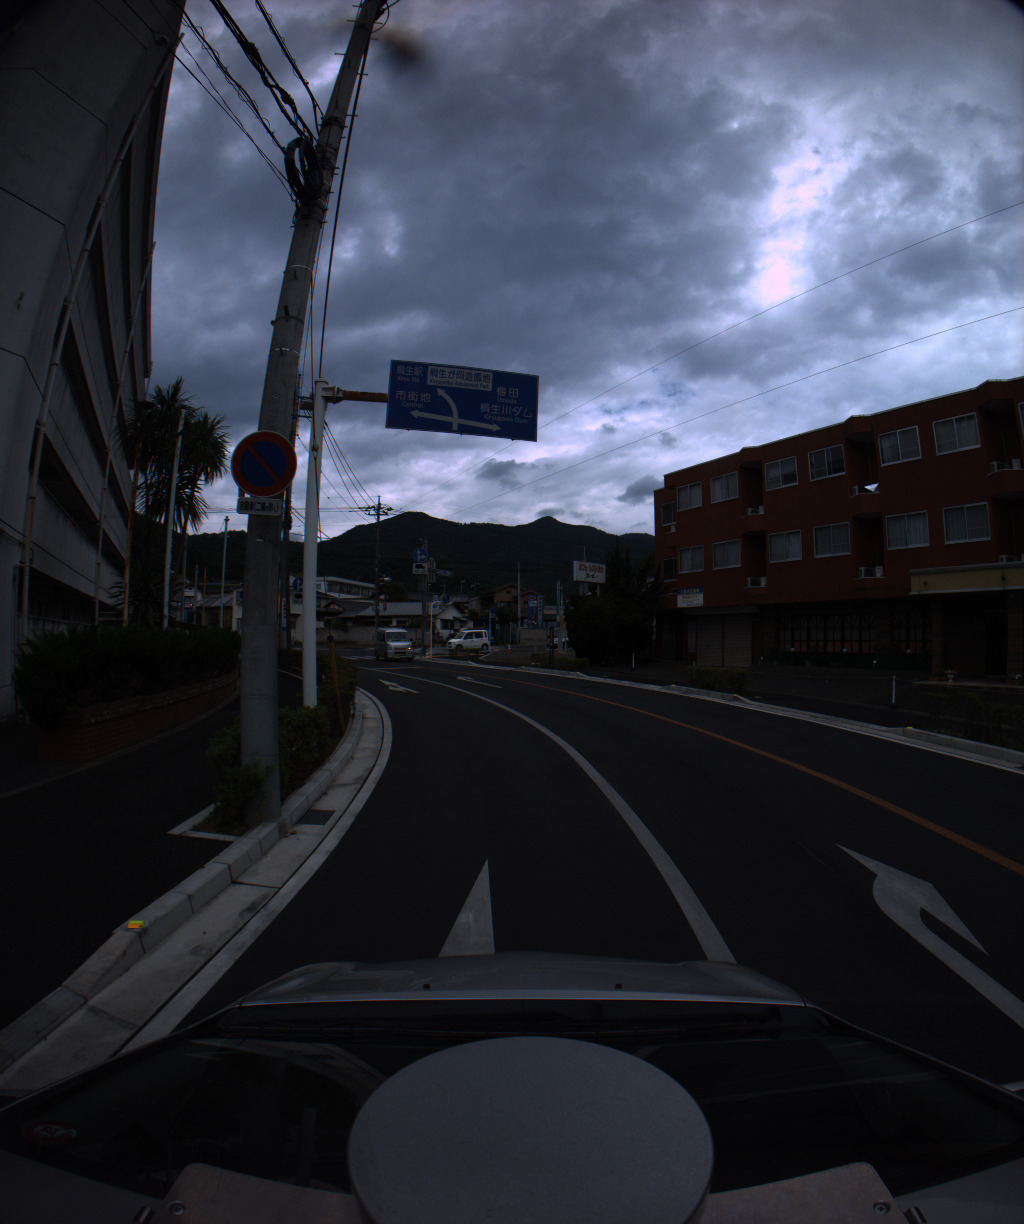
\includegraphics[pagebox=cropbox, scale=0.15]{sotuken_png/Test00_000314.jpg}
      \subcaption{曇りの時の風景画像}
      \label{Test00}
    \end{minipage}
    &
    \begin{minipage}[b]{0.32\linewidth}
      \centering
      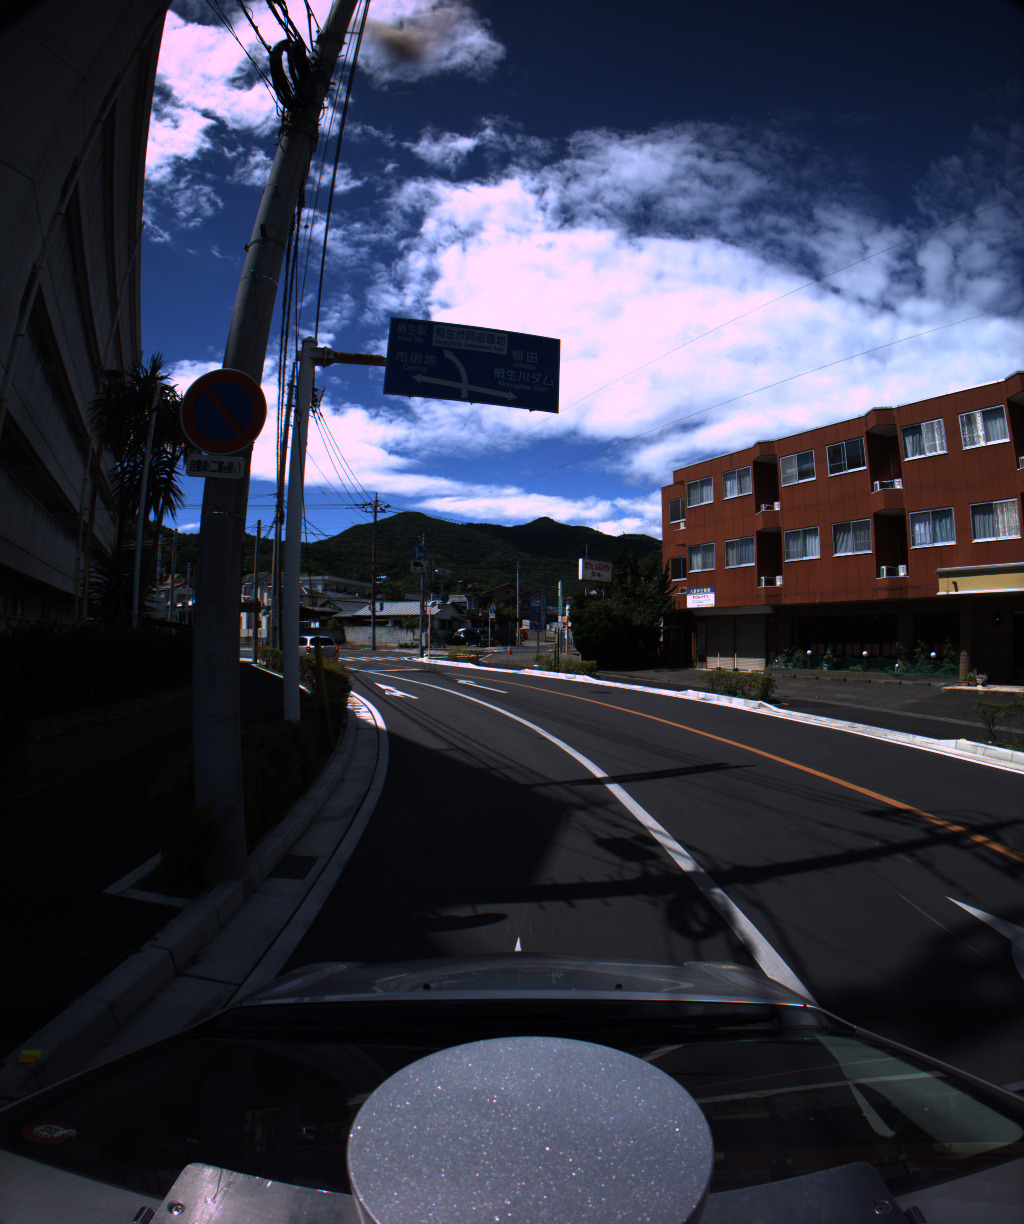
\includegraphics[pagebox=cropbox, scale=0.15]{sotuken_png/Test01_000133.jpg}
      \subcaption{晴れの時の風景画像}
      \label{Test01}
    \end{minipage}
  \end{tabular}
  \caption{風景画像}
  \label{view}
\end{figure}
シーンマッチングでは、シーンと呼ばれる風景画像を使用する。(図\ref{view})
風景画像には不変的な情報と可変的な情報の2種類の情報が描画されている。
不変的な情報とは、建物や遠景に見える山の輪郭、道路の形状など数時間単位等では決して変化することのない情報をさす。
可変的な情報とは、天候や時間などの影響による、雲の動きや画像全体の明度の変化等が相当する。(図\ref{Test00})
風景画像はこの天候や時間等の影響を受けやすい画像であるため、こういった変化に強い画像特徴を使用することで影響をなくす必要がある。

そこで、今回風景画像を照合する前にいくつかの画像特徴を使用した前処理を行う事で、どの画像特徴を使用した時が
天候や時間の影響を受けずに自己位置推定を行えるかを調べていく。

\subsection{自己位置推定}
\begin{figure}[t]
  \centering
  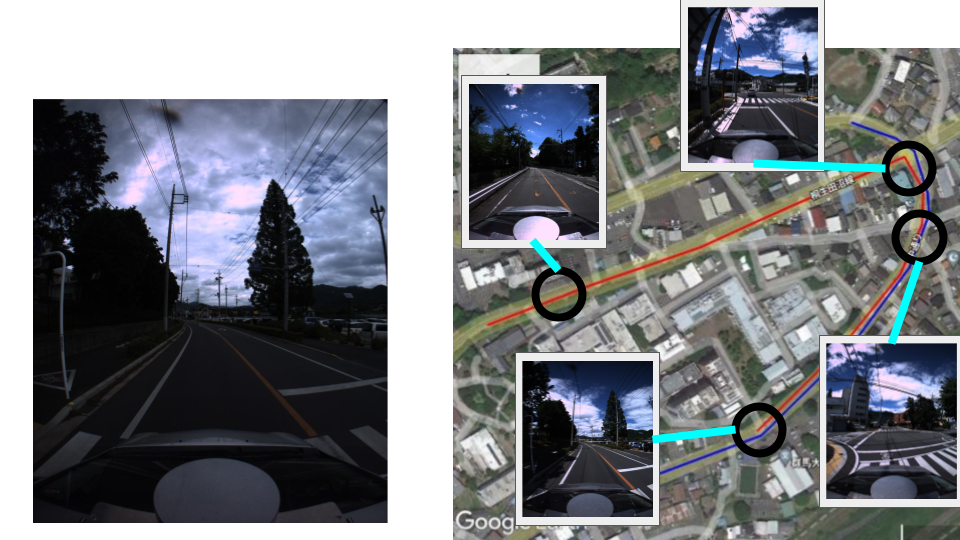
\includegraphics[pagebox=cropbox, scale=0.4]{sotuken_png/positioning.png}
  \caption{自己位置推定のイメージ}
  \label{positioning}
\end{figure}
自動運転車両が自動運転中に自己位置推定を行う方法はいくつかある。その中でも今回使用するのは風景画像を使った自己位置推定である。
風景画像を使った自己位置推定では、自動運転走行するルートの風景画像を事前に走行して撮影しておく。
そして、実際に走行しながら取得した画像と照らし合わせながら自分の位置を推定していく。
例えば、走行しながら取得した画像がA地点で撮影した画像と照合し同じと判断された場合、その取得した画像によって自動運転車両は自分の位置がA地点にあると推定することができる。
取得した画像と事前走行で得られた風景画像を照合する手法としてテンプレートマッチングを使用する。

また、テンプレートマッチングを行う際の処理として、以下の処理を行う。
\begin{enumerate}
  \item 0.1倍のスケールに画像縮小してマッチング
  \item サイズを変えずにCannyのエッジ検出をしてマッチング
  \item 0.1倍のスケールに画像縮小しCannyのエッジ検出をしてマッチング
  \item サイズを変えずにLBP特徴を計算してマッチング
  \item 0.1倍のスケールに画像縮小してLBP特徴を計算してマッチング
  \item サイズを変えずにHOG特徴を計算してマッチング
\end{enumerate}
それぞれの前処理を行うことで画像に特徴を持たせることができ、似ている画像同士の類似度を高めることができると予想した。
使用した画像処理技術については次節にて説明する。

\subsection{テンプレートマッチング}
\begin{figure}[t]
  \centering
  \begin{tabular}{lr}
    \begin{minipage}[b]{0.5\linewidth}
      \centering
      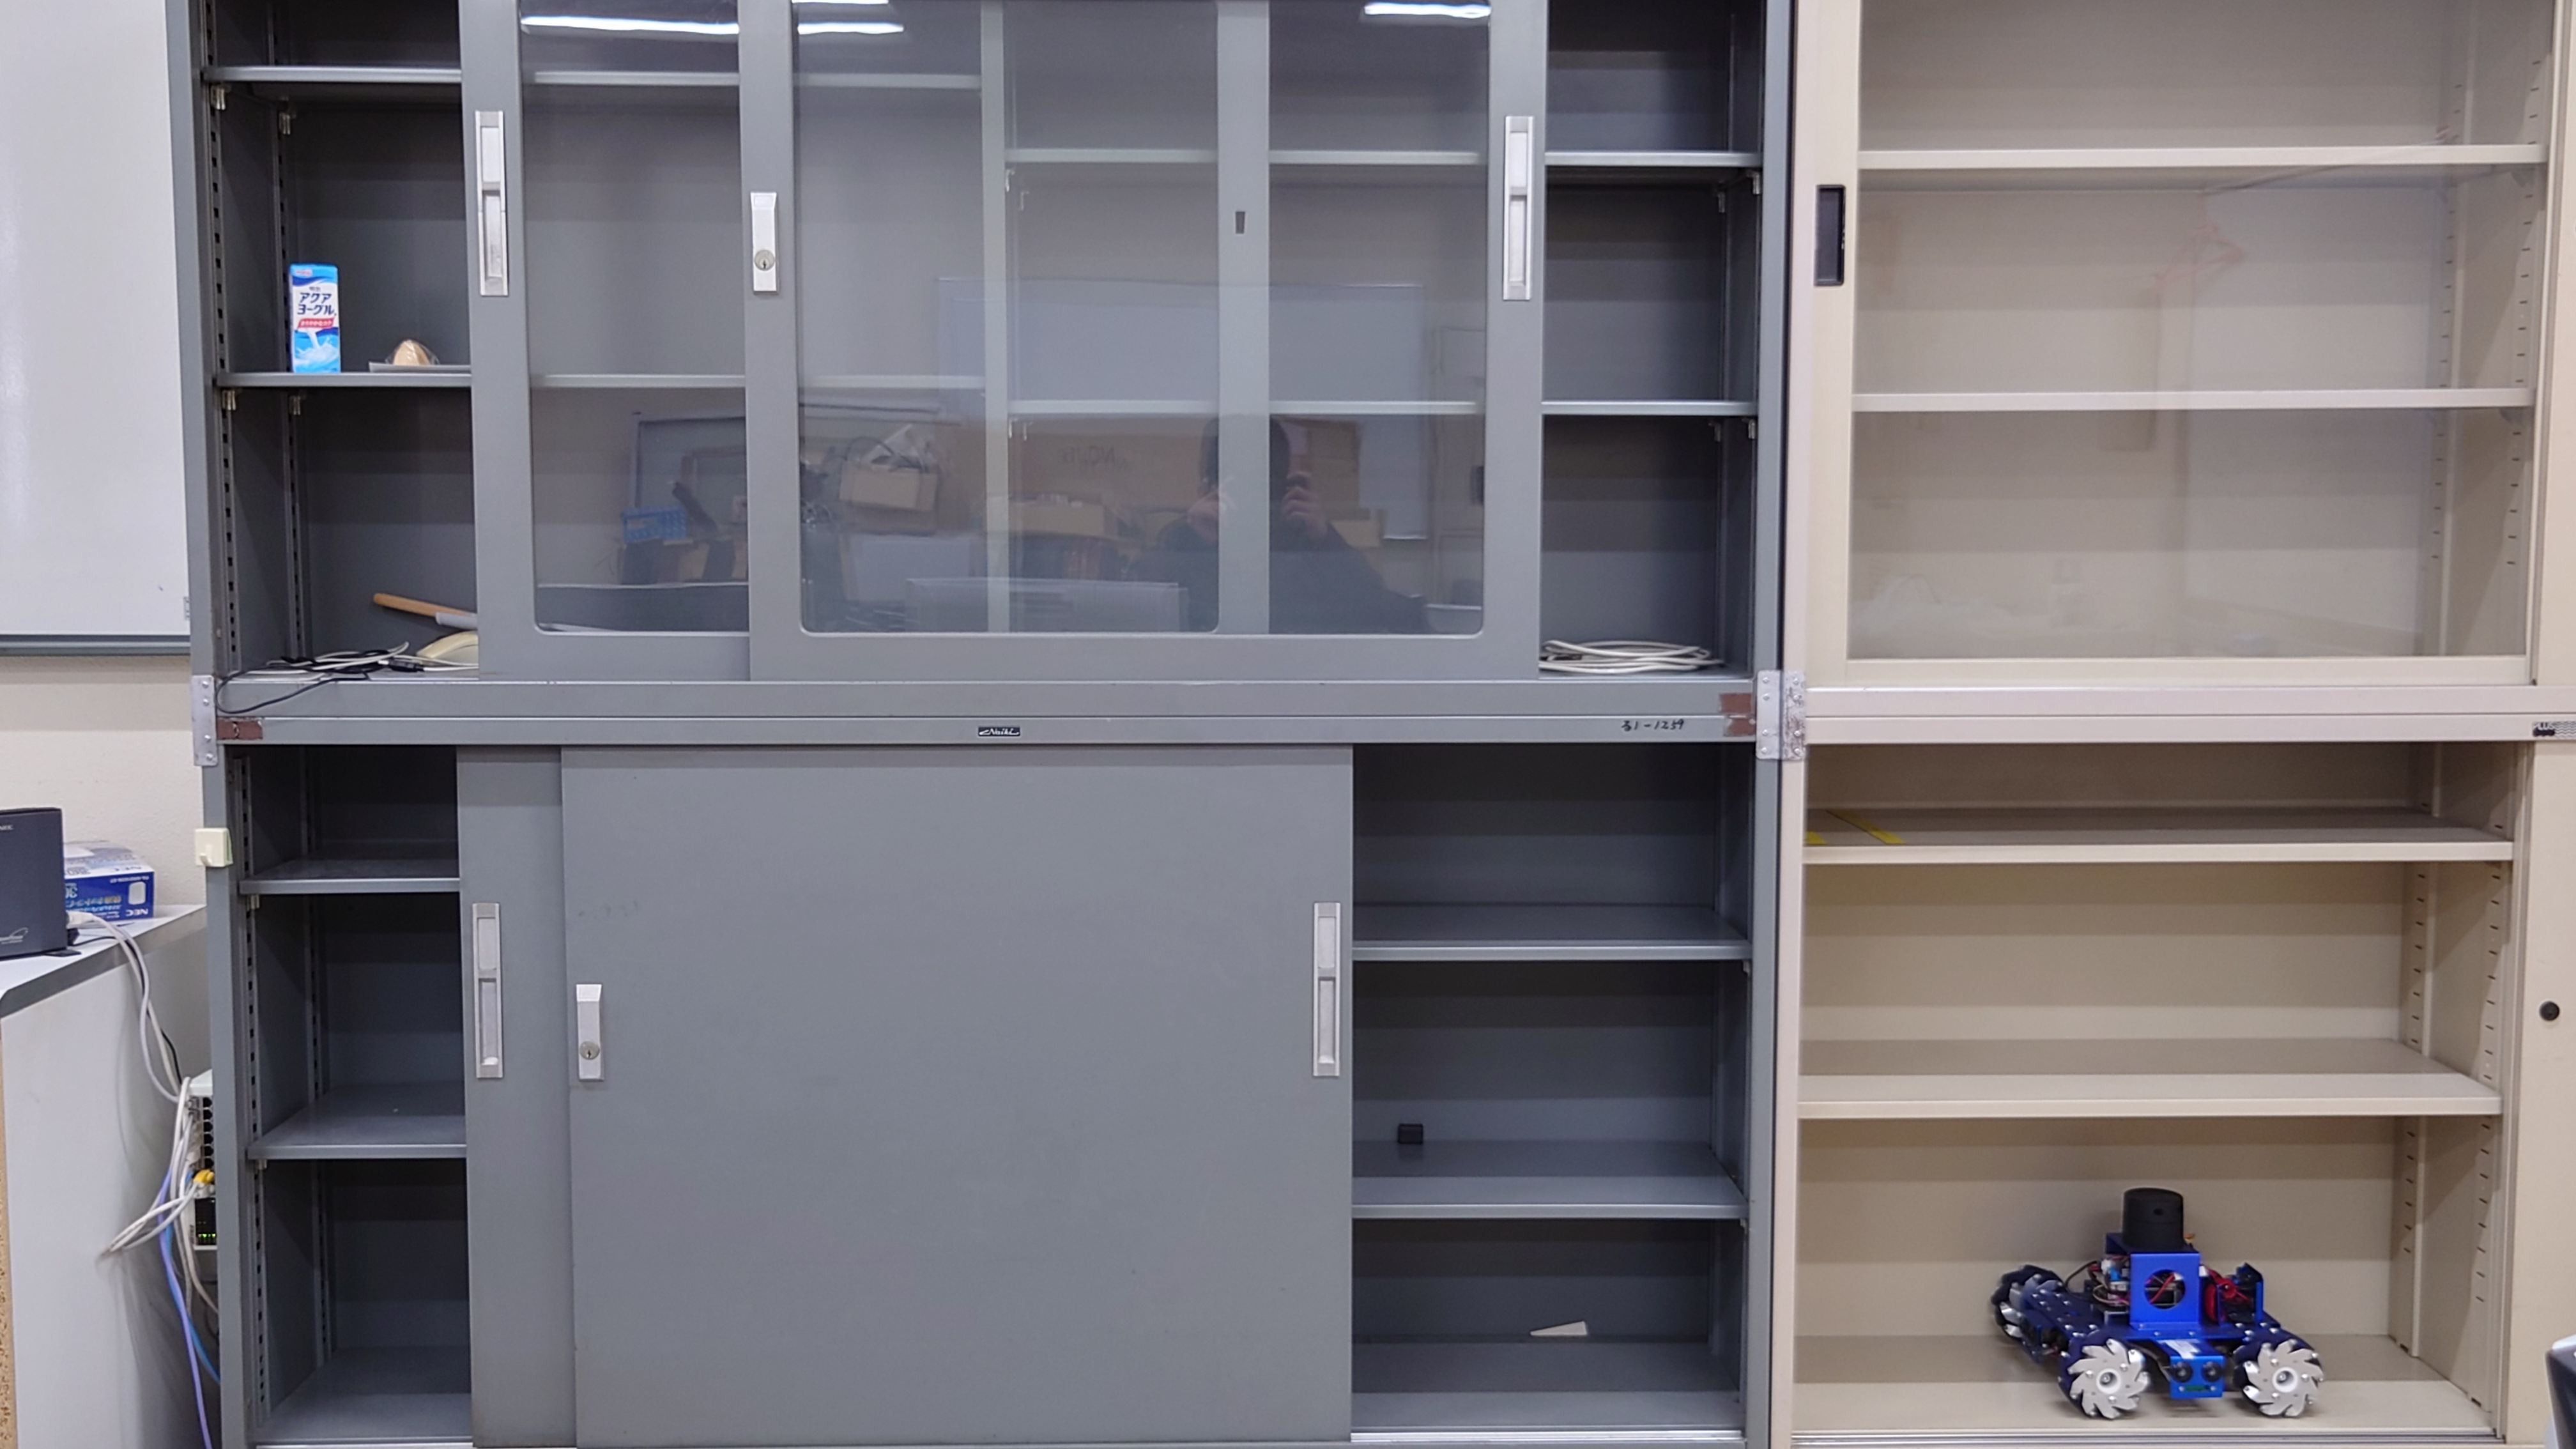
\includegraphics[pagebox=cropbox, scale=0.05]{BasedImage.JPG}
      \subcaption{探索対象画像}
      \label{BasedImage}
    \end{minipage}
     &
    \begin{minipage}[b]{0.5\linewidth}
      \centering
      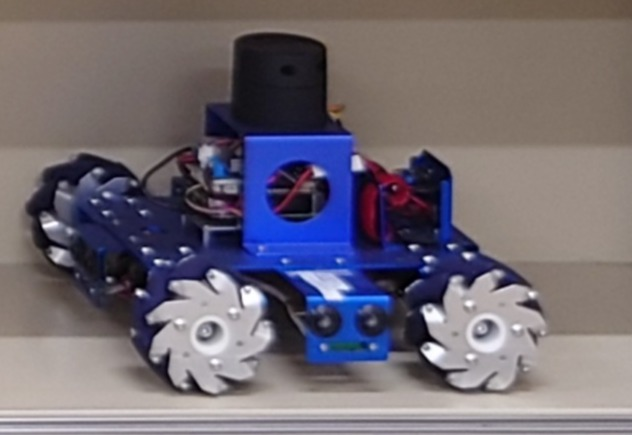
\includegraphics[pagebox=cropbox, scale=0.3]{TemplateImage.jpeg}
      \subcaption{テンプレート画像}
      \label{TemplateImage}
    \end{minipage}
  \end{tabular}  
  \caption{テンプレートマッチングに必要な画像}
  \label{}
\end{figure}
\begin{figure}[t]
  \centering
  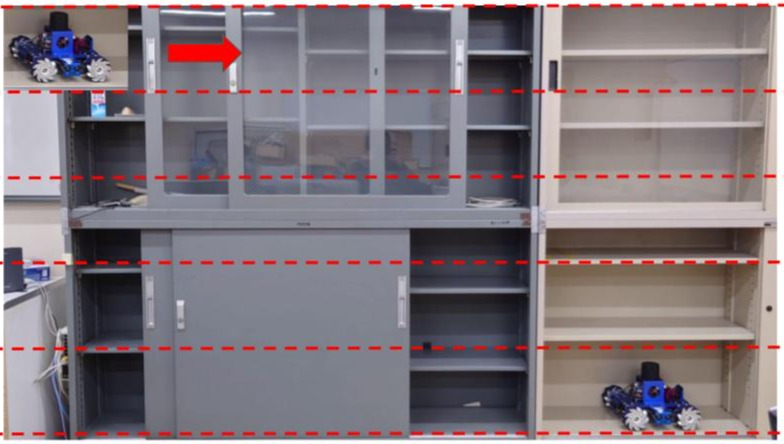
\includegraphics[pagebox=cropbox, scale=0.42]{TemplateMatching.jpeg}
  \caption{テンプレートマッチングの動作イメージ}
  \label{TemplateMatching}
\end{figure}


テンプレートマッチングとは、画像同士の類似度を調べる画像処理である。
テンプレートマッチングを行うにあたってまずテンプレート画像と探索対象画像と呼ばれる二つの画像を用意する必要がある。
テンプレート画像とは、探索対象画像中で探し出したい画像情報が大きく描かれた画像のことである。(図\ref{TemplateImage})
また、テンプレート画像の画像サイズは探索対象画像よりも小さいことが必要である。
探索対象画像とは、テンプレート画像に描かれた画像情報とどれだけ類似しているかを調べたい画像のことである。(図\ref{BasedImage})
探索対象画像内にはテンプレート画像と同じ画像情報が必ずしも含まれている必要性はない。

テンプレートマッチングでは画像同士の類似度を調べる手法がいくつか存在するが、ここでは実験でも使用したZNCC(零平均正規化相互相関)について説明する。
$I(i,j)$が探索対象画像の座標$(i,j)$における画素値、$T(i,j)$がテンプレート画像の座標$(i,j)$における画素値とする。
また、テンプレート画像の解像度を$M\times N$とする。このとき、ZNCCは次の式で求めることができる。
\begin{align}
  ZNCC \: = & \frac{\Sigma^{N-1}_{j=0}\:\Sigma^{M-1}_{i=0} \left(I(i,j)\:-\: \overline{I}\right) \left(T(i,j)\:-\:\overline{T}\right)}{\sqrt{\Sigma^{N-1}_{j=0}\:\Sigma^{M-1}_{i=0} \left(I(i,j)\:-\: \overline{I}\right)^2 \:\times\:\Sigma^{N-1}_{j=0}\:\Sigma^{M-1}_{i=0} \left(T(i,j)\:-\:\overline{T}\right)^2}}
\end{align}
ここで$\overline{I}$と$\overline{T}$はそれぞれ探索対象画像とテンプレート画像の画素値の平均値となる。

ZNCCのもととなったNCC(正規化相互相関)があり、NCCはベクトルの内積の式と同一なのでZNCCは計算結果が1に近づくほど類似度が高くなる。
NCCとの違いは画像全体から全画素の平均値を引くことでノイズや明るさの影響を受けにくいという利点がある。

これらの画像と類似度計算を使ってマッチングを行う。テンプレートマッチングでは探索対象画像の左上の画素にテンプレート画像を合わせ、
その画素からテンプレート画像と同じサイズの領域とテンプレート画像で類似度を調べる。その結果の値をその画素の類似度とする。
これを探索対象画像上を走査しながら行っていく。(図\ref{TemplateMatching})その後、一番大きい類似度を持った画素がマッチングされが部分となる。

\subsection{画像縮小}
0.1倍スケールに縮小した画像を使ってマッチングを行った理由としては、
画像のスケールを下げることで細かい部分のノイズを削減し大まかな形状を得ることができるためである。
解像度が高い画像では、木々の揺れや葉の色、タイルの網目などの細かい情報が散乱している。
その状態でテンプレートマッチングを行った場合、そういった細かい情報まで一致しなければ類似の画像として扱うことができない。
風景画像では、遠方の山や建物の輪郭といった大まかな物体の形が分かればよいので、細かい情報をなくす簡単な処理としてスケールの縮小を行った。
また、画像のスケールを縮小することでテンプレートマッチングの走査領域が減るため、実行時間を削減することができる効果もある。

\subsection{エッジ検出}
\begin{figure}[t]
  \centering
  \begin{tabular}{cc}
    \begin{minipage}[b]{0.32\linewidth}
      \centering
      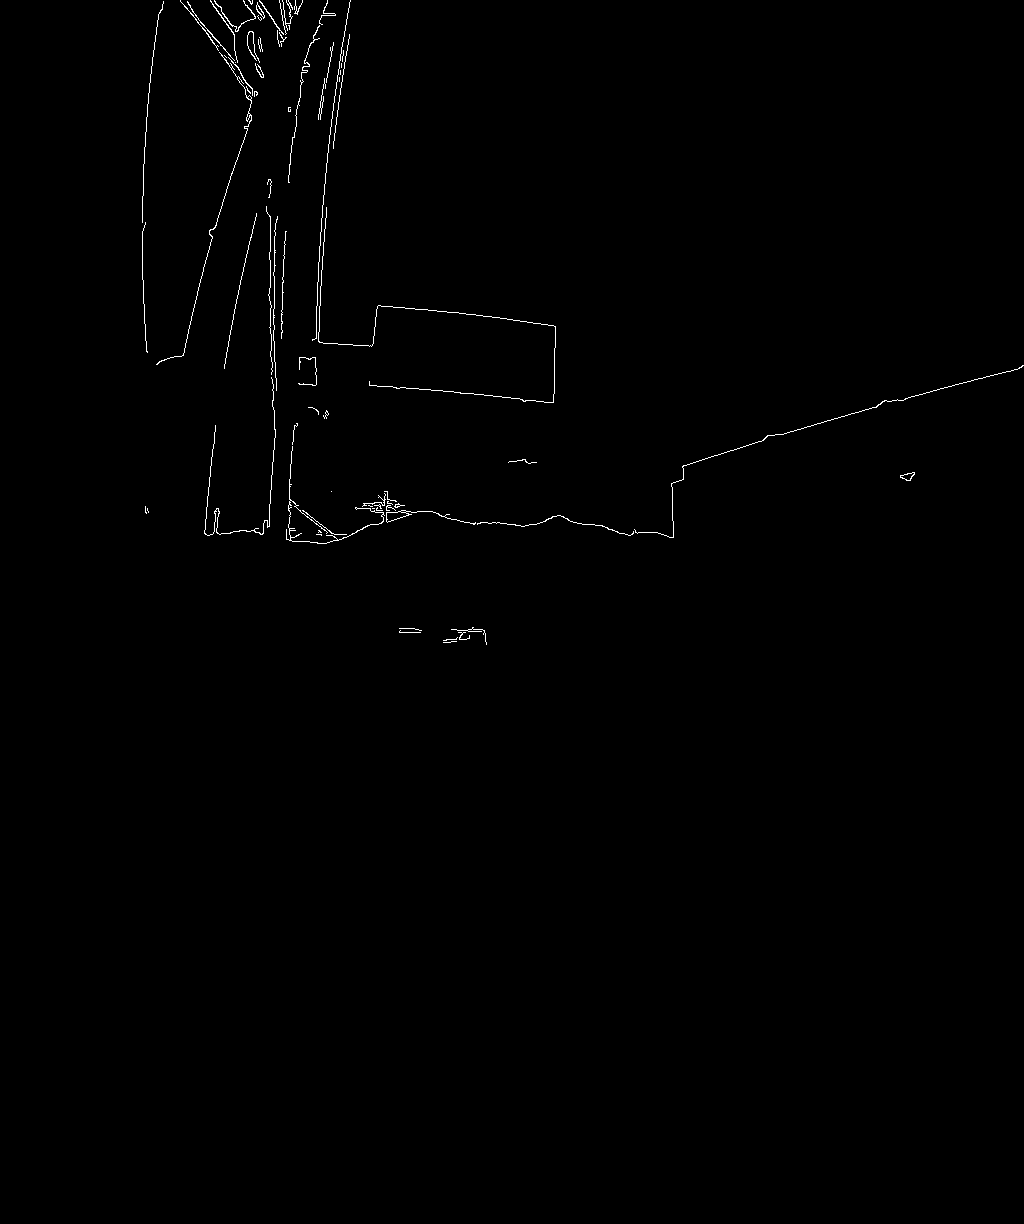
\includegraphics[pagebox=cropbox, scale=0.15]{sotuken_png/canny.png}
      \subcaption{曇りの時のエッジ特徴}
      \label{dstCAN}
    \end{minipage}
    &
    \begin{minipage}[b]{0.32\linewidth}
      \centering
      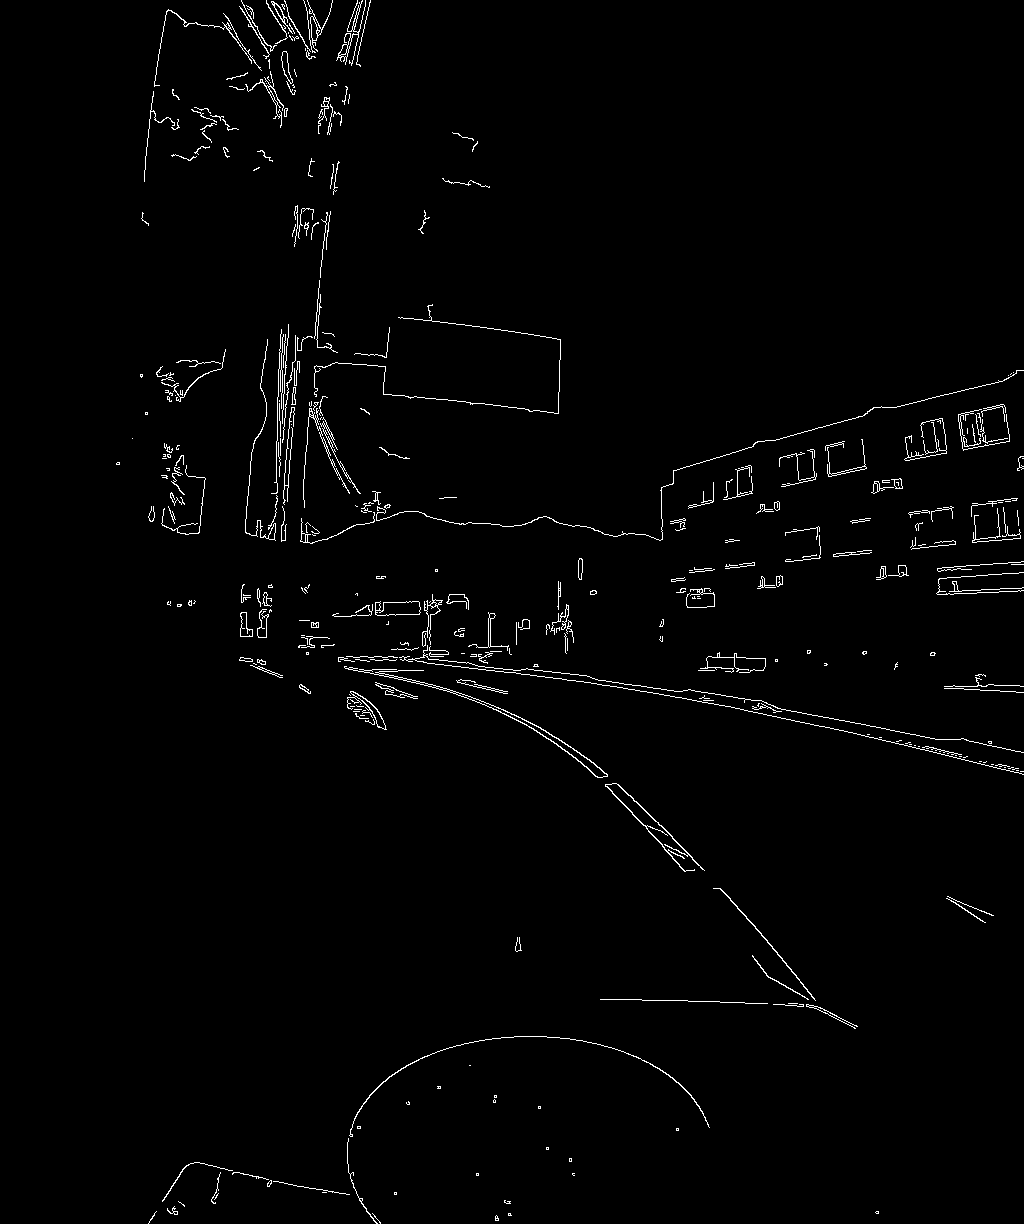
\includegraphics[pagebox=cropbox, scale=0.15]{sotuken_png/canny2.png}
      \subcaption{晴れの時のエッジ徳亮}
      \label{dstCAN}
    \end{minipage}
  \end{tabular}
  \caption{風景画像に対してエッジ検出を適用した場合}
  \label{CANimg}
\end{figure}

エッジ検出とは、画像内の物体の輪郭や輝度差が閾値以上の部分のみを抽出する画像処理のことである。
基本的にエッジは輝度の不連続な部分であり、明るいところから極端に暗いところ、暗いところから極端に明るくなるところにエッジができやすい。
ここでは、いくつかあるエッジ検出のひとつであるCanny法について説明する。

Canny法ではいくつかの処理に分けてエッジ検出を行っていく。
まず、入力画像にグレースケール化を行い、その入力画像にガウシアンフィルタをかける。この時、ガウシアンフィルタをかけた画像をGとする。
ガウシアンフィルタとは加重平均フィルタと呼ばれ、注目画素からの距離に応じて重み付けを行いその合計を画素値とするフィルタの事である。
ガウシアンフィルタをかけて画像を平滑化することで、画像内のノイズを消去、軽減する目的がある。

次に、画像GにSobelフィルタをかけてx方向とy方向の一次微分画像$G_x$,$G_y$を求める。
Sobelフィルタもエッジ検出法の一つで、入力画像に対しx方向かy方向に一次微分を行いx方向であれば縦線、y方向であれば横線のエッジを検出する。

先ほど用いた$G_x,G_y$を使って、エッジ強度と勾配方向を求めていく。
エッジ強度$I$と勾配方向$\theta$は次の式で求めることができる。
\begin{align}
  I(i,j)\: =  & \sqrt{G_x(i,j)^2 + G_y(i,j)^2} \\
  \theta \: = & \arctan{\frac{G_y}{G_x}}
\end{align}

次に、先ほど求めたエッジの勾配を使って非極大抑制と呼ばれる処理を行う。非極大抑制とは注目している画素値がその画素のエッジ勾配方向に隣接している
2つの画素値と比べて極大値であるかどうかを調べる。極大値であればそのまま残し、非極大値であればその画素はエッジでないため画素値を0とする。

最後に先ほどの非極大抑制処理で得られたエッジが正しいかどうか調べるために、ヒステリシス閾値処理を行う。
ヒステリシス閾値処理では、まず最大閾値と最小閾値の二つの閾値を決定する。そして、非極大抑制で残ったエッジを最大閾値を以上のエッジ、
最小閾値以上最大閾値未満のエッジ、最小閾値に満たないエッジの3つに分ける。
最小閾値に満たない場合はそのエッジをエッジとみなさず消去する。
最小閾値以上最大閾値未満のエッジの場合は、そのエッジをエッジの断片または始点と考える。その後、そのエッジに隣接するエッジを全て調べる。
調べた中に最大閾値以上のエッジが存在するのであれば、始点から終点までのエッジの集合をエッジとする。
最大閾値以上のエッジが存在しない場合、そのエッジの集合はエッジとみなさず消去する。

以上の処理を繰り返すことで画像内のエッジを検出するのがCanny法である。\cite{f4}

今回の実験でCannyのエッジ検出を前処理で用いる理由としては、Cannyのエッジ検出では導出でも説明したがヒステリシス閾値処理の
おかげで弱いエッジを消すことができ、雲の模様や電線などの細い線等をある程度消すことができる。
そのため、建物や山の輪郭線のような強いエッジのみ残すことができ
テンプレートマッチングを行った際に一致している時と一致していない時での類似度に差が出ると予想した。
\subsection{LBP特徴}
\begin{figure}[t]
  \centering
  \begin{tabular}{cc}
    \begin{minipage}[b]{0.5\linewidth}
      \centering
      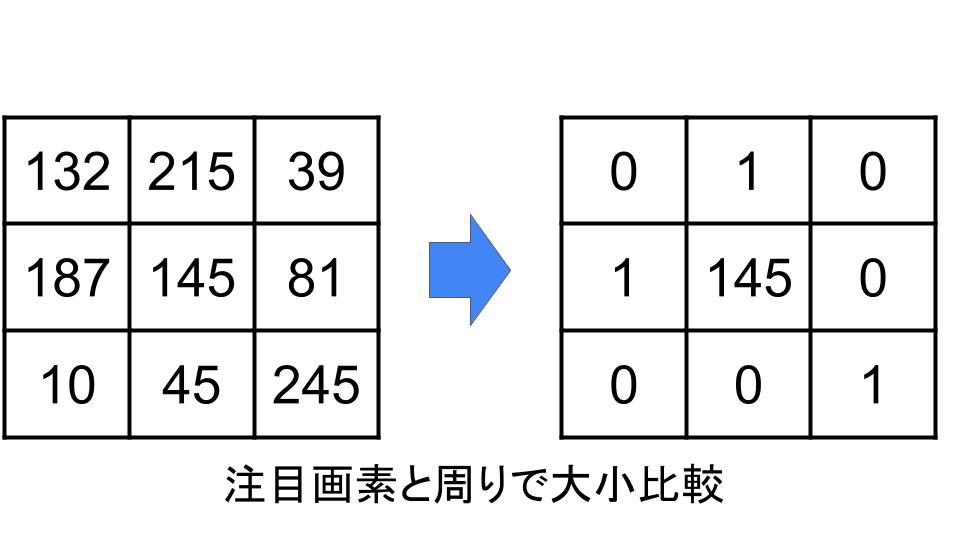
\includegraphics[pagebox=cropbox, scale=0.25]{LBP.jpg}
    \end{minipage}
    &
    \begin{minipage}[b]{0.5\linewidth}
      \centering
      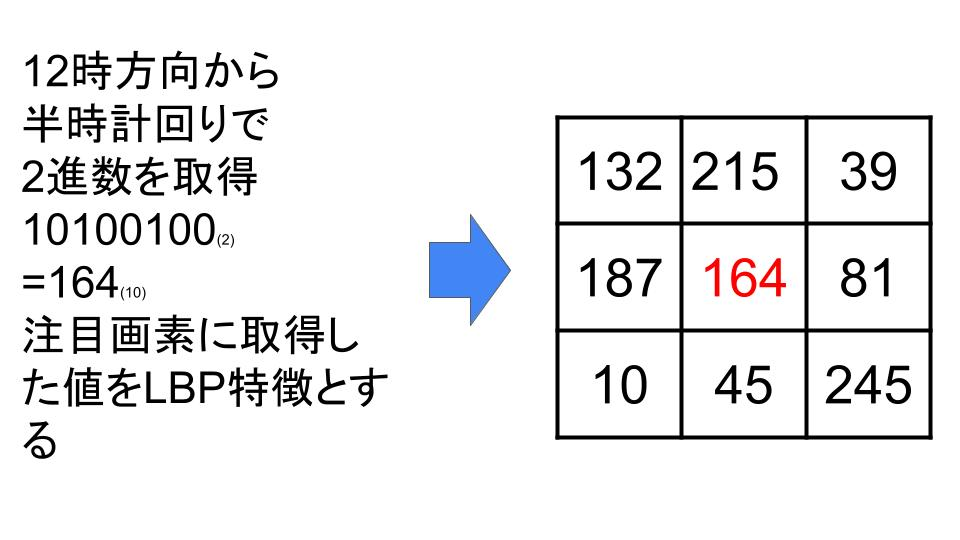
\includegraphics[pagebox=cropbox, scale=0.25]{LBP2.jpg}
    \end{minipage}
  \end{tabular}
  \caption{LBP特徴の求め方}
  \label{LBP}  
\end{figure}

\begin{figure}[t]
  \centering
  \begin{tabular}{cc}
    \begin{minipage}[b]{0.5\linewidth}
      \centering
      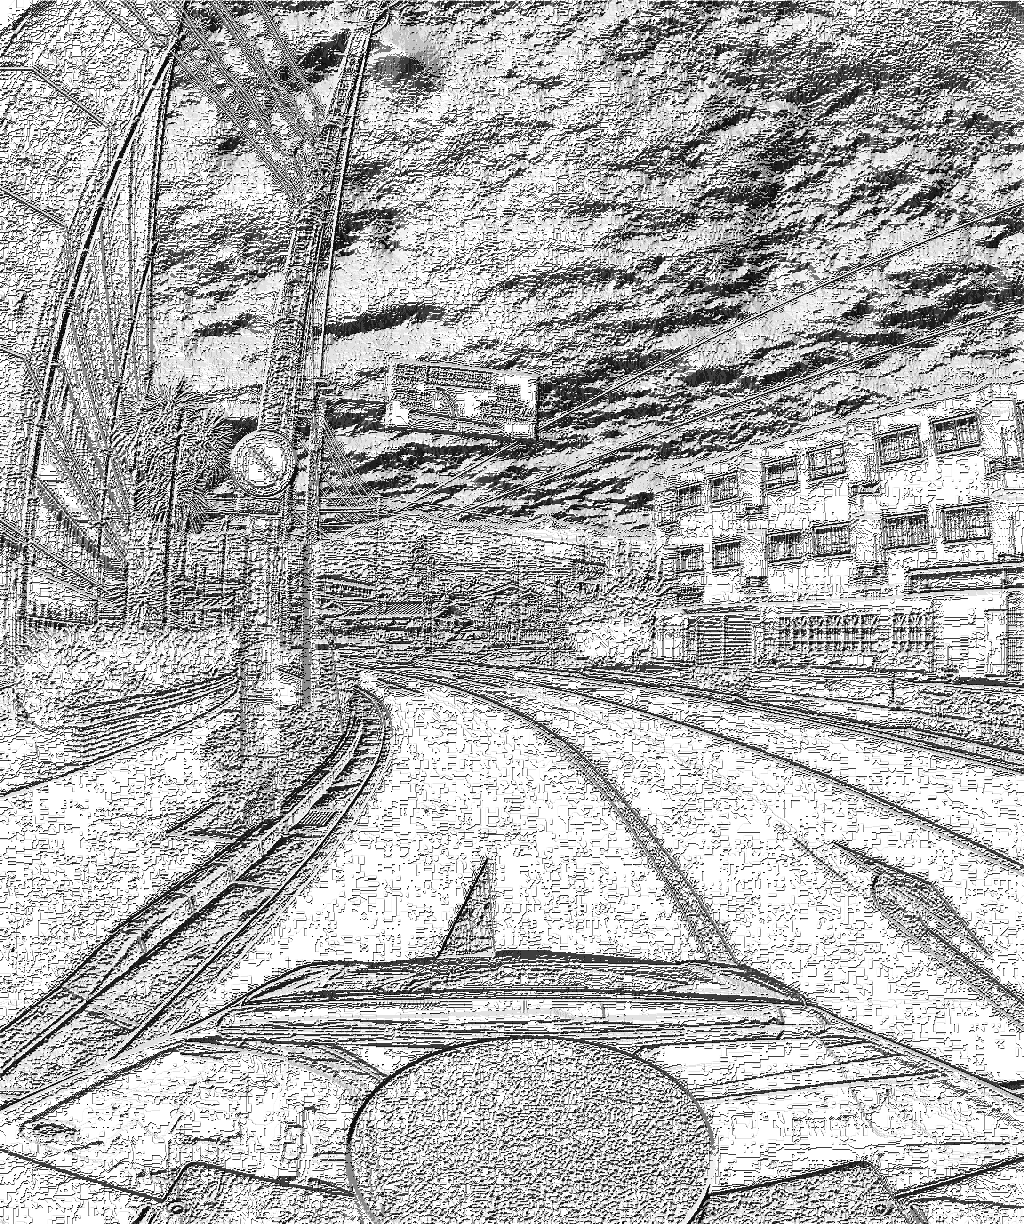
\includegraphics[pagebox=cropbox, scale=0.15]{sotuken_png/dst_LBP.png}
      \subcaption{曇りの画像にLBP特徴}
      \label{dstLBP}
    \end{minipage}
    &
    \begin{minipage}[b]{0.5\linewidth}
      \centering
      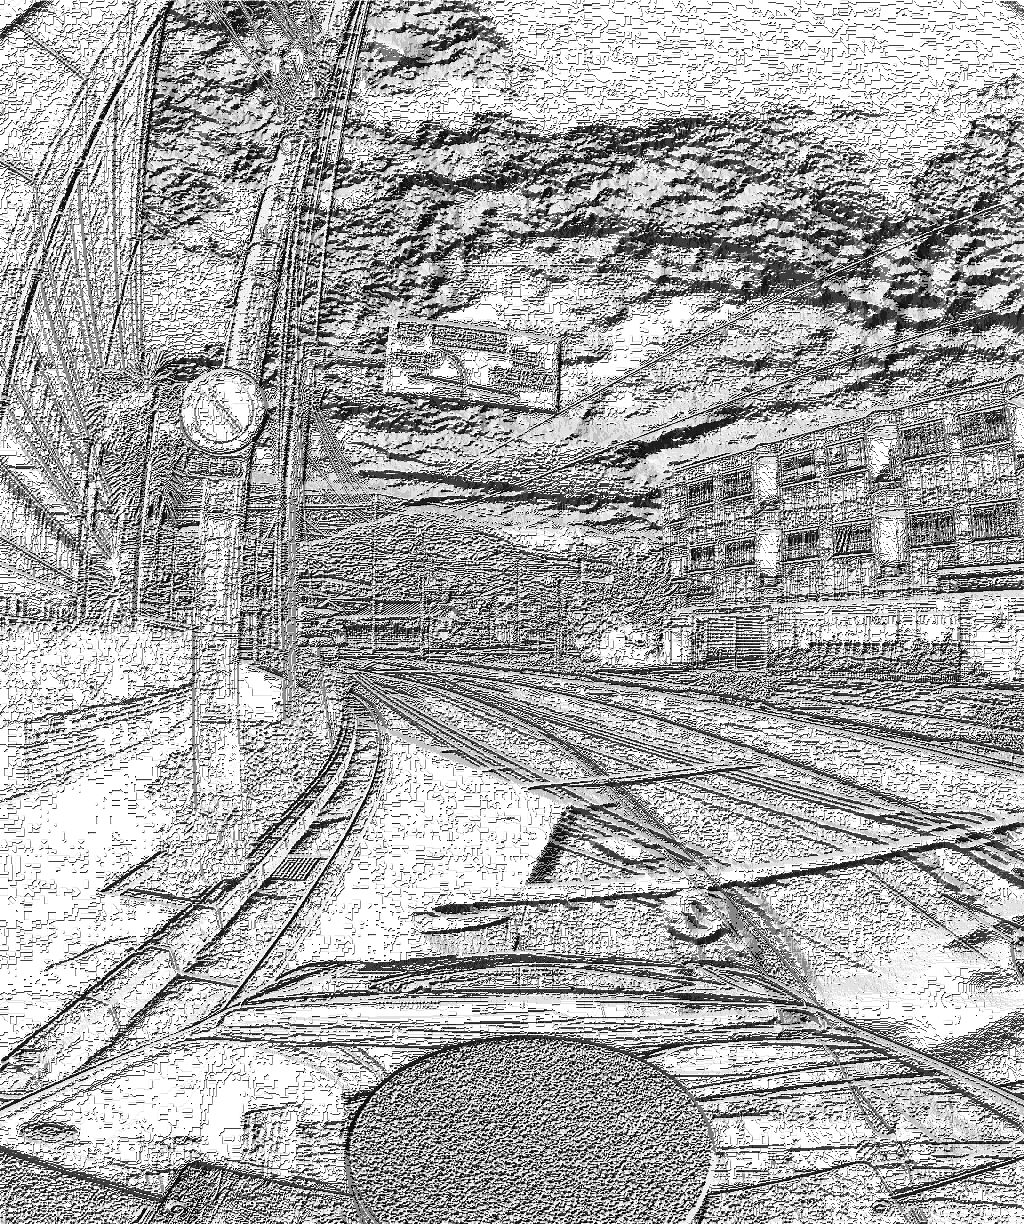
\includegraphics[pagebox=cropbox, scale=0.15]{sotuken_png/dst_LBP2.png}
      \subcaption{晴れの画像にLBP特徴}
      \label{dstLBP2}
    \end{minipage}
  \end{tabular}
  \caption{LBP特徴を適用した画像}
  \label{LBPimg}  
\end{figure}
LBP特徴(Local Binaly Ptterns)とは、画像特徴量の一つで注目画素とその周りの輝度のパターンを特徴とするものである。
LBP特徴は、まず入力画像にグレースケール化を行う。その後、注目画素とその周り八近傍に存在する画素の画素値を比較する。
比較した結果注目画素よりも近傍に存在する画素の方が画素値が大きいのであればば1、小さければ0とする。
その後、注目画素に対して12時方向に存在する画素から反時計回りに1週0,1の値を取得する。
取得したその値を2進数に置き換えて得られた値が、注目画素のLBP特徴となる。
例えば、図\ref{LBP}のように中心の画素値が144の場合、八近傍に存在する画素値をそれぞれ144よりも大きければ1、小さければ0とする。
こうして0と1に振りなおされた八近傍の中から注目画素の12時方向から反統計周りに値を取得していく。
今回の例でいえば、12時方向の値は1でありここから反時計回りに取っていくと、10100100が得られる。
10100100を10進数に直すと164となり、これが注目画素のLBP特徴値となる。\cite{f5}

LBP特徴は、注目画素とその周りの八近傍の画素値との相対的な輝度差によって得られるため、
画像全体の明るさやコントラストが変化したとしてもLBP特徴は変化しにくく、
画像に対して回転などの線形変換が行われたとしても2進数のパターンがシフトするだけで
全体的なLBP特徴の変化は少ない。

今回の実験でLBP特徴を使った理由としては、風景画像には目印となる建物や山といった変化の少ない情報のほかに、天候や時間帯による明度の変化など
の常に変化する周りの環境の情報も含まれる。前処理なしで晴れの日の画像と曇りの日の画像でテンプレートマッチングを行った場合、快晴の空と曇りの空で
差が出てしまいマッチングが上手くいかないことがある。そこでLBP特徴を使うことで快晴と曇りのコントラストの差をある程度取ることができ、
さらに画像のスケールを縮小することでさらに差を取ることができる。\subsection{HOG特徴}
\begin{figure}[t]
  \centering
  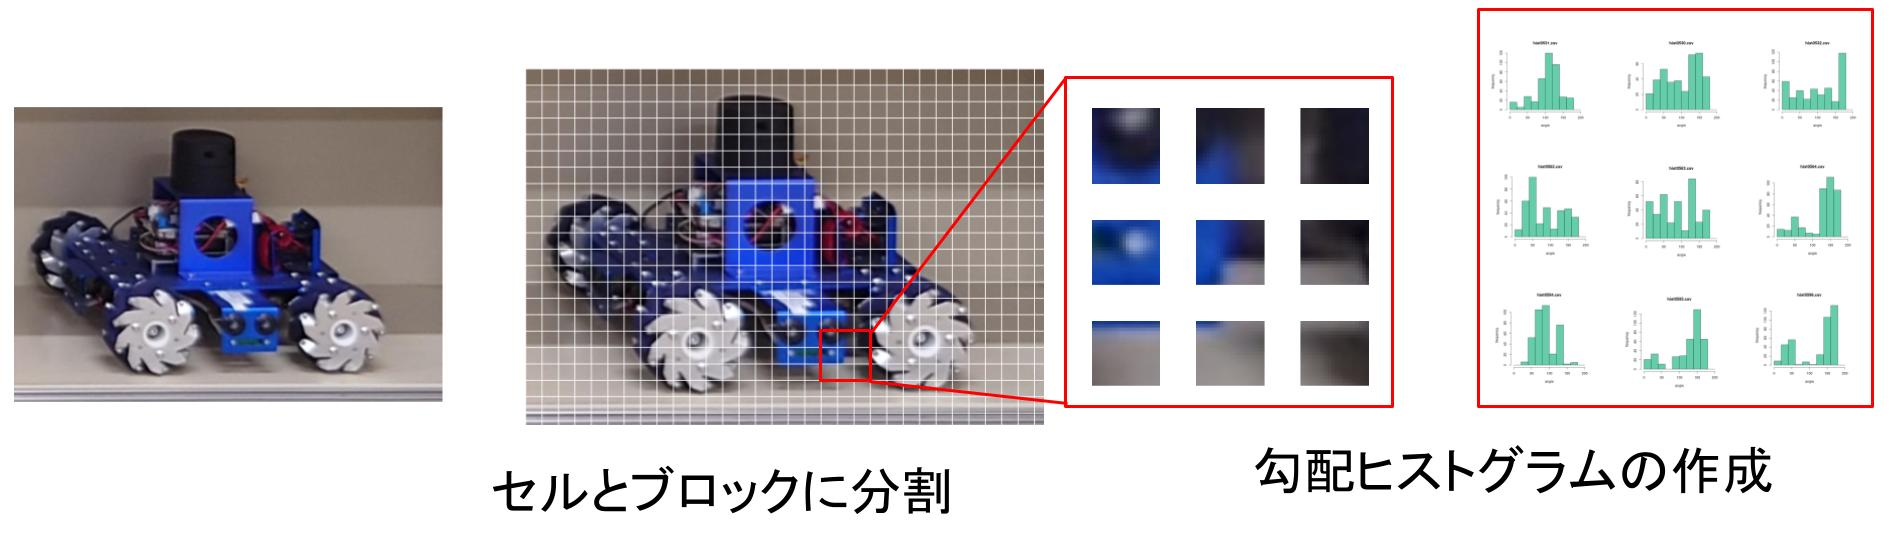
\includegraphics[pagebox=cropbox, scale=0.2]{HOG.jpg}
  \caption{HOG特徴の導出}
  \label{HOG}
\end{figure}

\begin{figure}[t]
  \centering
  \begin{tabular}{cc}
    \begin{minipage}[b]{0.5\linewidth}
      \centering
      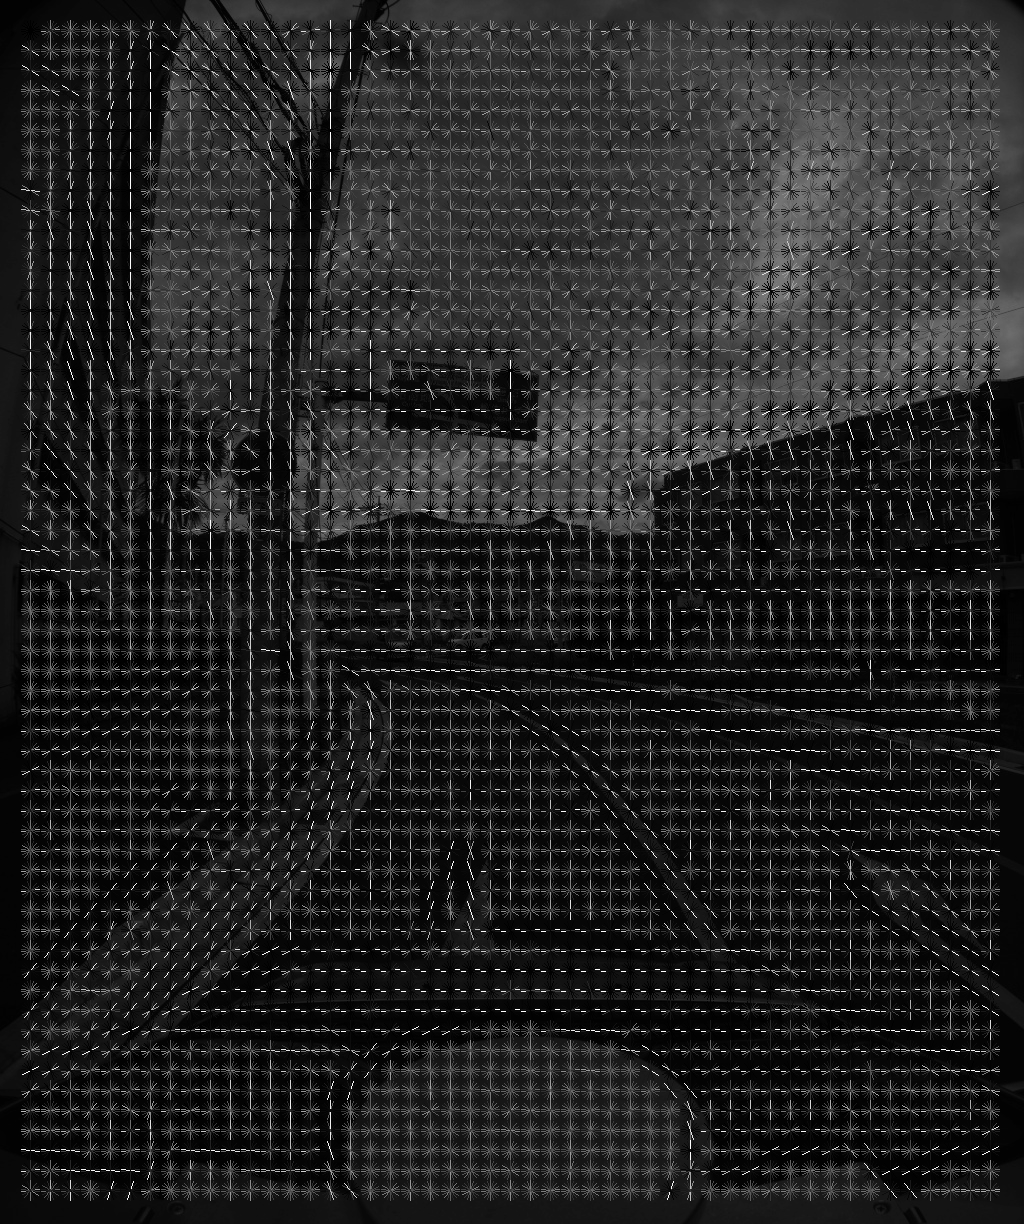
\includegraphics[pagebox=cropbox, scale=0.15]{sotuken_png/dst_HOG.png}
      \subcaption{曇りの画像にHOG特徴}
      \label{dstHOg}
    \end{minipage}
    &
    \begin{minipage}[b]{0.5\linewidth}
      \centering
      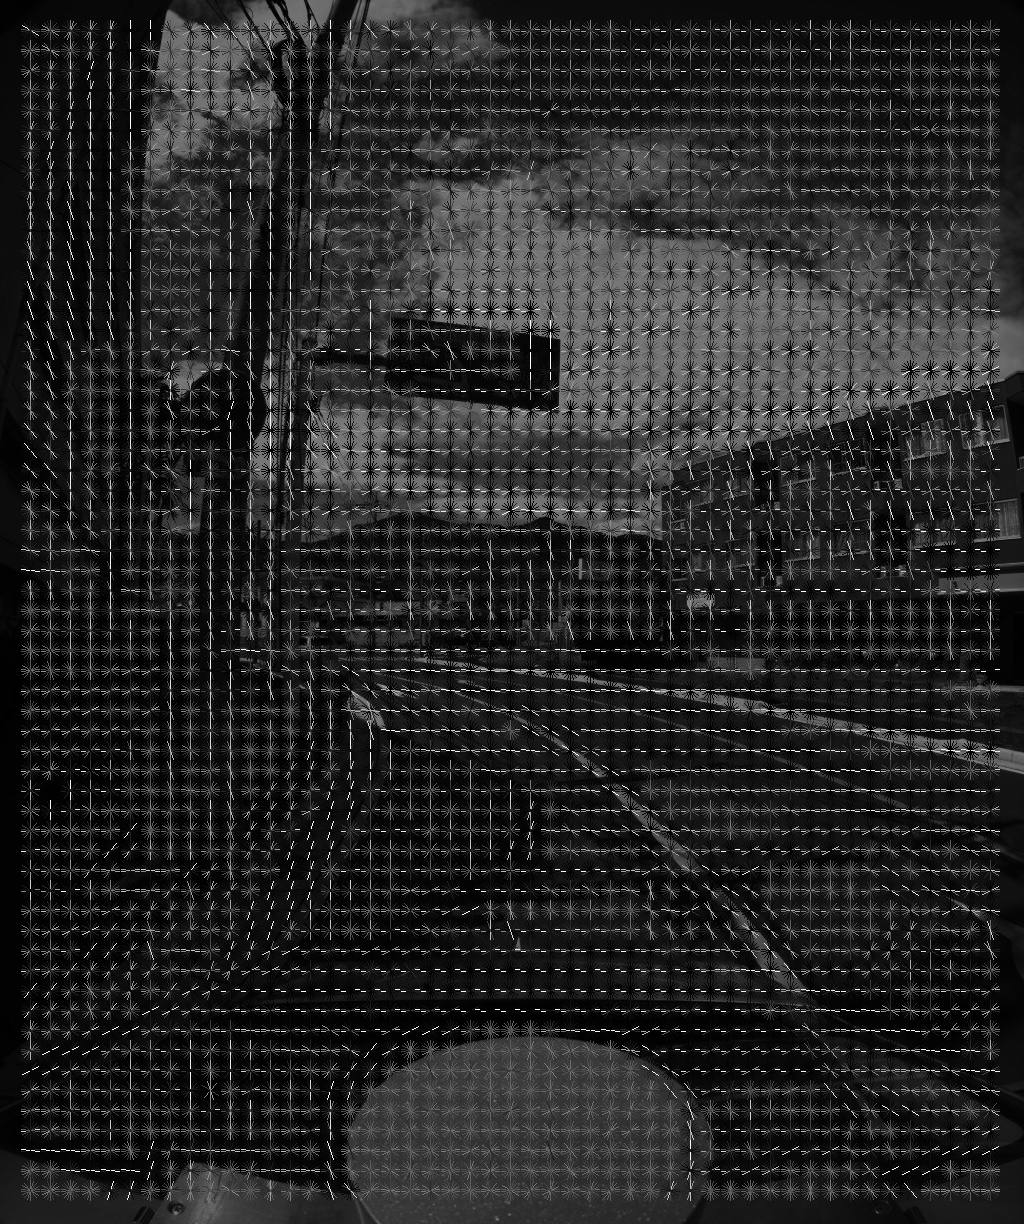
\includegraphics[pagebox=cropbox, scale=0.15]{sotuken_png/dst_HOG2.png}
      \caption{晴れの画像にHOG特徴}
      \label{dstHOG2}
    \end{minipage}
  \end{tabular}
  \caption{HOG特徴を適用した結果}
  \label{HOGimg}
\end{figure}

HOG特徴とは、LBP特徴と同じ画像特徴の一つで入力画像の輝度勾配ヒストグラムを特徴するものである。
HOG特徴の求め方は、まず入力画像にグレースケール化を行った後、いくつかのピクセルが集まってできたセルと
セルがいくつか集まってできたブロックに分ける。今回の実験では1セル20$\times$20ピクセルとし、1ブロック3$\times$3のセルの集合とした。
次に1ブロックに含まれるセルごとの強度と輝度勾配を計算する。
今回、プログラムの実行時間を少なくするために積分ヒストグラムを使用した。\cite{f6}
強度と輝度勾配を求めるためにCannyのエッジ検出と同様に画像に対してx方向とy方向に対してSobelフィルタをかけていく。
強度と輝度勾配の式は(2)、(3)式を使用する。
その後、セル毎にセル内の輝度勾配のヒストグラムを作成(図\ref{HOG})し、それをブロック単位で連結しHOG特徴とする。\cite{f7}


HOG特徴は、画像の特定領域内の輝度勾配を用いるので物体の形状を表現することができ、SVMと使うことで人物検出や車両の検出などに用いられている。

今回の実験でHOG特徴を使用した理由としては、風景画像には建物や山のような目印となるものほかに道路の白線等の直線といった形状情報を
含んでいる。そういった、情報をより強調することができるのがHOG特徴である。前処理でHOG特徴を使用することで
テンプレートマッチングを行った際に一致している時と一致していない時での類似度に差が出ると予想した。

\subsection{実験の手法}

\begin{figure}[t]
  \centering
  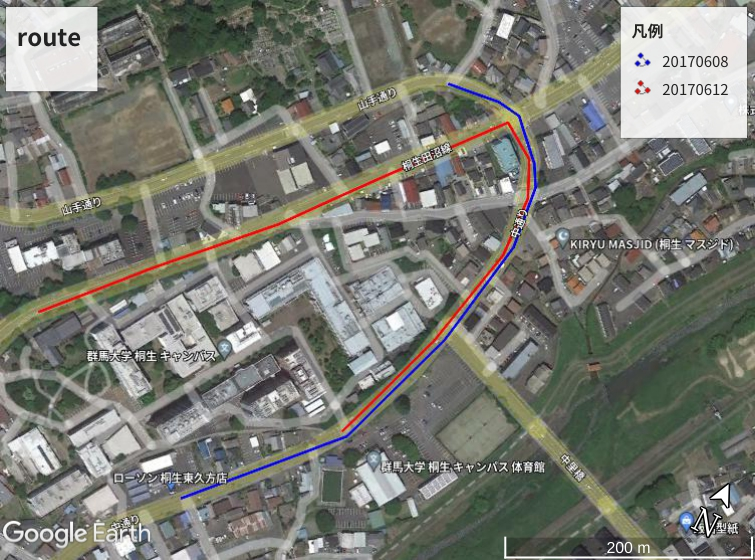
\includegraphics[pagebox=cropbox, scale=0.6]{route.jpg}
  \caption{群馬大学周りの走行ルート}
  \label{route}
\end{figure}
今回の実験では、群馬大学周りのコースを走行したときの風景画像を使用して自己位置推定を行い画像毎の類似度のピークの調査と精度検証を行った。
風景画像は2種類あり、2017年6月8日に撮影されたもの671枚(以後青ルートと呼称する)と2017年6月12日に撮影されたもの490枚(以後赤ルートと呼称する)がある。
今回、青いルートの画像を探索対象画像とし赤いルートの画像をテンプレート画像とした。
これらの画像を使って節で説明した前処理を行いテンプレートマッチングを行う。
まず、青ルートの0フレーム目の画像に対して赤ルートの0フレーム目から489フレーム目までの画像を使ってテンプレートマッチングをおこないそれぞれの類似度を求める。
この処理を青ルートの670フレーム目までの画像に対して同様の処理を行う。
これによって青ルートのnフレーム目は赤ルートのmフレーム目に類似度のピークが来るといったことがわかる。

精度検証で用いる式は次の式を用いた。
\begin{align}
  accuracy &= \frac{ピーク時の類似度の値}{ピーク時の類似度の値 + 2番目に高い類似度の値}
\end{align}
この式によりaccuracyが1に近づくほどピークが突出して高く、0.5に近づくほど他に似たようなピークが出現しているということがわかる。
この検証式を用いる理由としては、自己位置推定を行う際にピークの類似度と似ている値が多く出現した場合、
誤った風景画像が結果として出力されてしまう。そのため、ピーク時の値がほかの値よりも突出しているのであれば突出している程よく、
誤った風景画像が出力されるのを防ぐことができる。

\section{結論}
\subsection{実験の結果}
\begin{figure}[H]
  \centering
  \begin{tabular}{cc}
    \begin{minipage}[b]{0.5\linewidth}
      \centering
      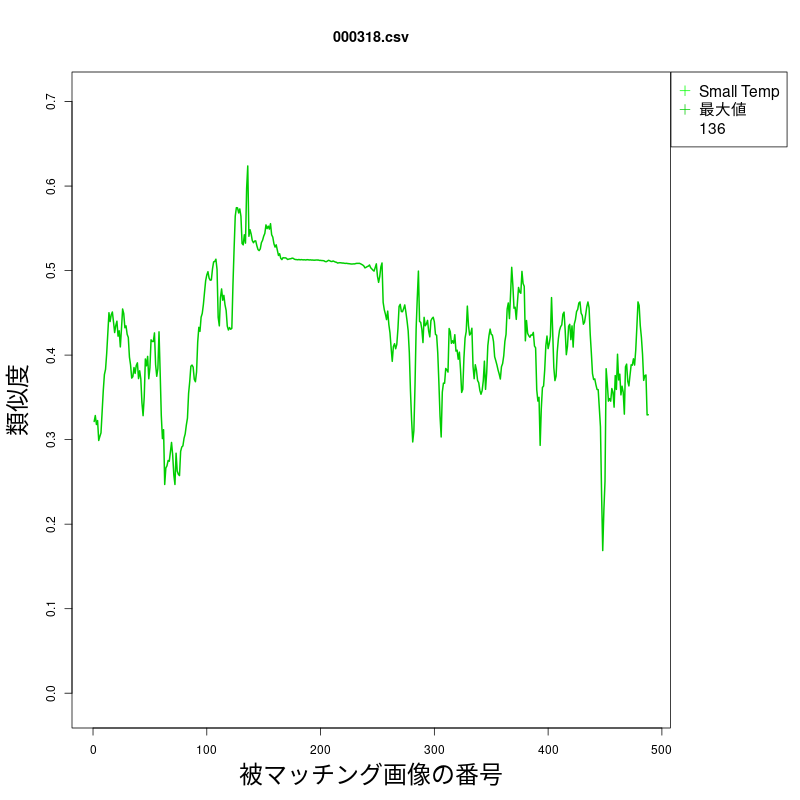
\includegraphics[pagebox=cropbox, scale=0.25]{sotuken_png/resulttemp_000318.png}
    \end{minipage}
    &
    \begin{minipage}[b]{0.5\linewidth}
      \centering
      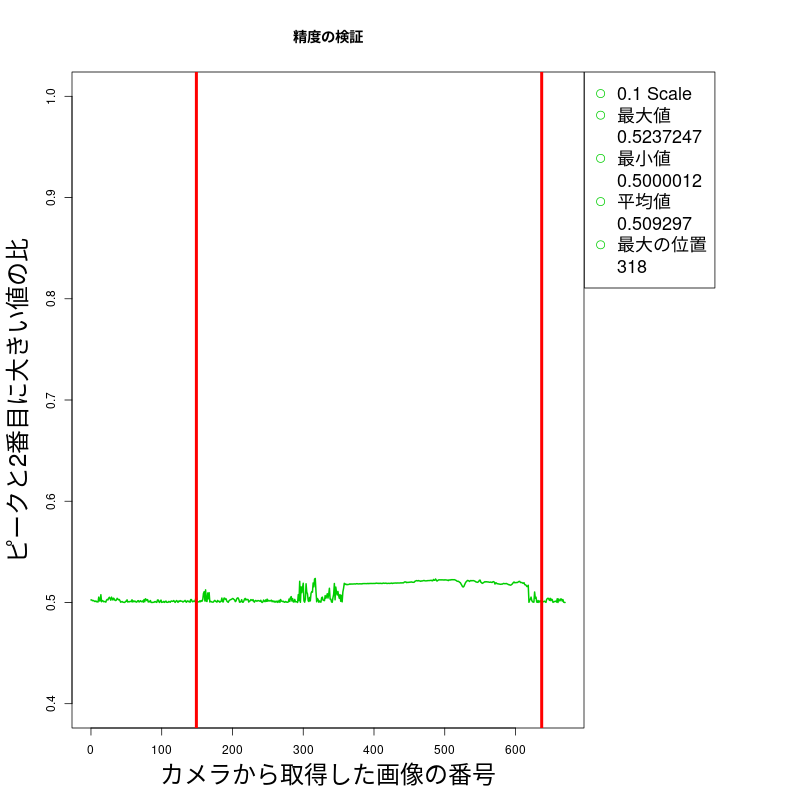
\includegraphics[pagebox=cropbox, scale=0.25]{sotuken_png/peak/peak_temp.png}
    \end{minipage}
  \end{tabular}
  \caption{画像縮小のみを行った時の自己位置推定の結果と精度検証}
  \label{tempR}

\end{figure}
\begin{figure}[H]
  \centering
  \begin{tabular}{cc}
    \begin{minipage}[b]{0.5\linewidth}
      \centering
      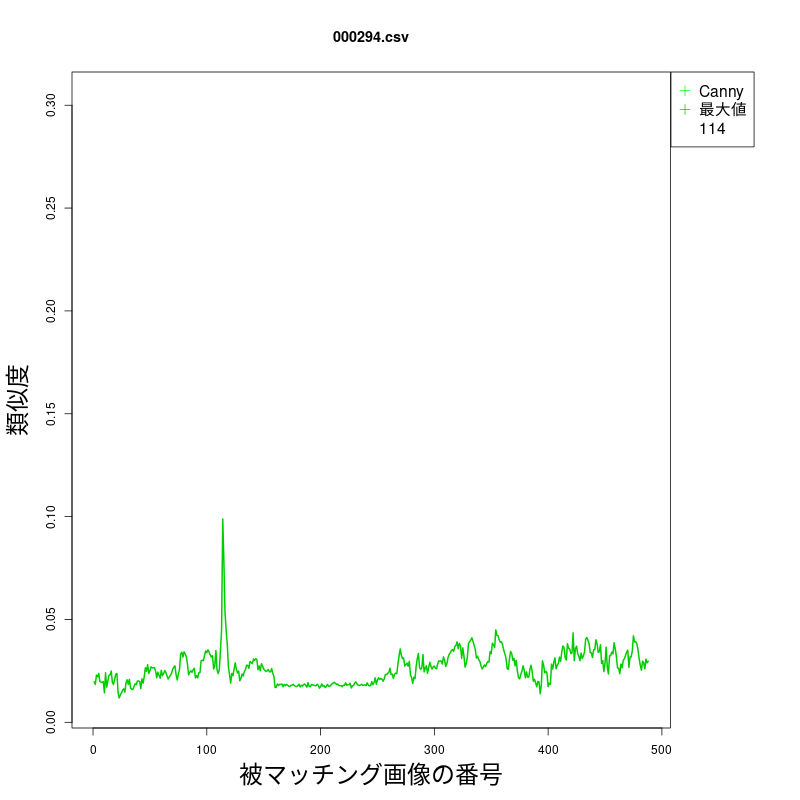
\includegraphics[pagebox=cropbox, scale=0.25]{sotuken_png/resultCanny_000294.png}
    \end{minipage}
    &
    \begin{minipage}[b]{0.5\linewidth}
      \centering
      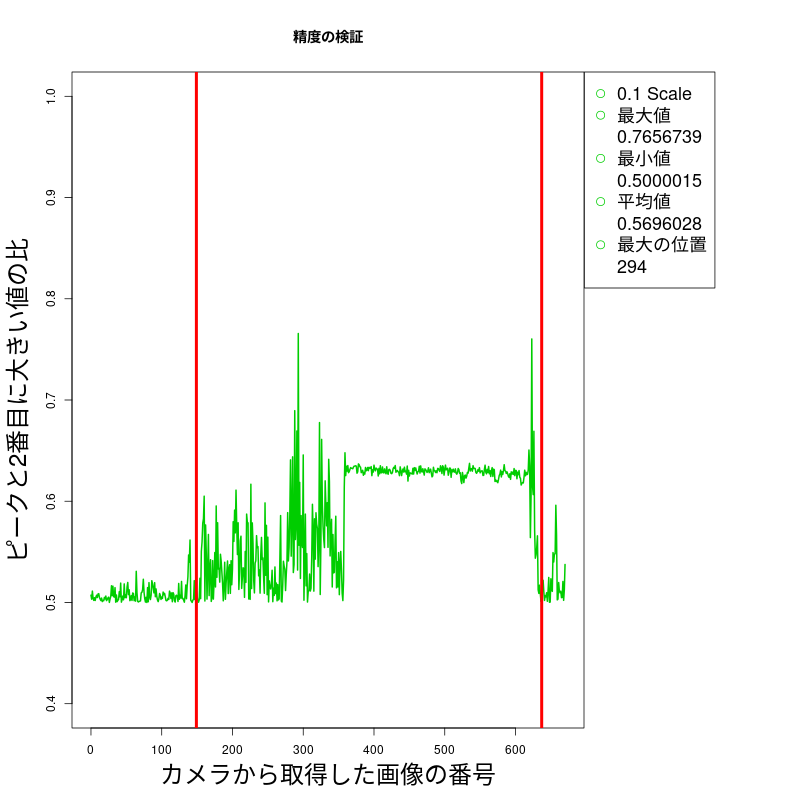
\includegraphics[pagebox=cropbox, scale=0.25]{sotuken_png/peak/peak_Canny.png}
    \end{minipage}
  \end{tabular}
  \caption{エッジ検出を行った時の自己位置推定の結果と精度検証}
  \label{CannyR}
\end{figure}

\begin{figure}[H]
  \centering
  \begin{tabular}{cc}
    \begin{minipage}[b]{0.5\linewidth}
      \centering
      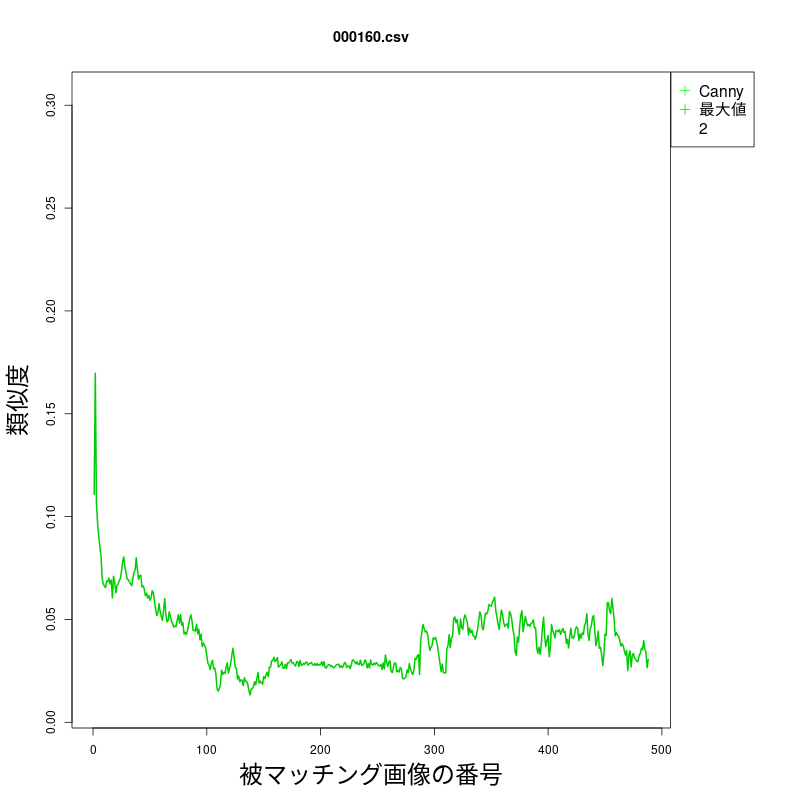
\includegraphics[pagebox=cropbox, scale=0.25]{sotuken_png/resultSCanny_000160.png}
    \end{minipage}
    &
    \begin{minipage}[b]{0.5\linewidth}
      \centering
      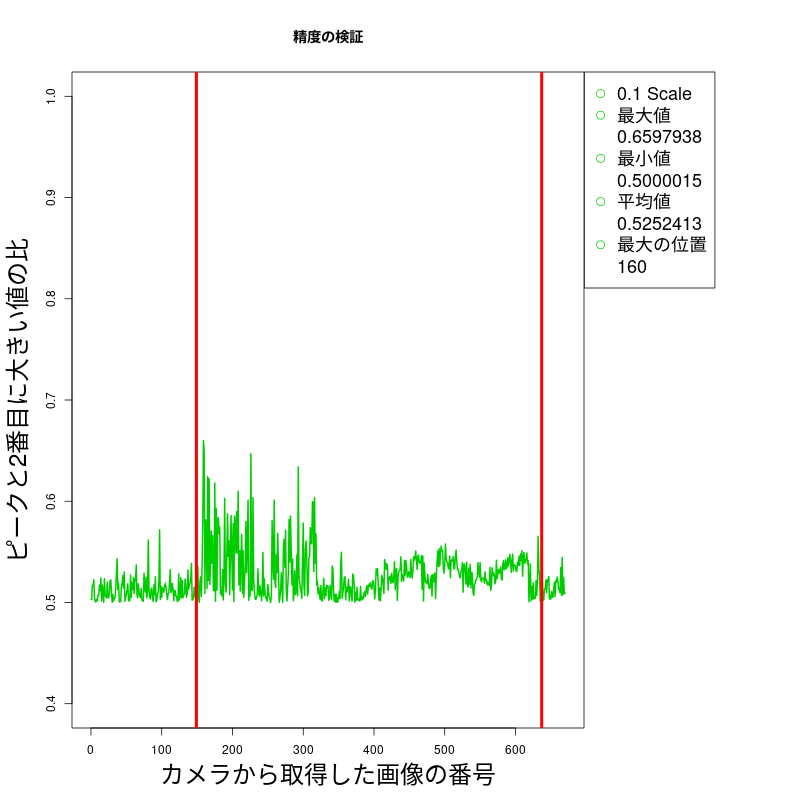
\includegraphics[pagebox=cropbox, scale=0.25]{sotuken_png/peak/peak_Canny_small.png}
    \end{minipage}
  \end{tabular}
  \caption{画像縮小とエッジ検出を行った時の自己位置推定の結果と精度検証}
  \label{SCannyR}
\end{figure}

\begin{figure}[H]
  \centering
  \begin{tabular}{cc}
    \begin{minipage}[b]{0.5\linewidth}
      \centering
      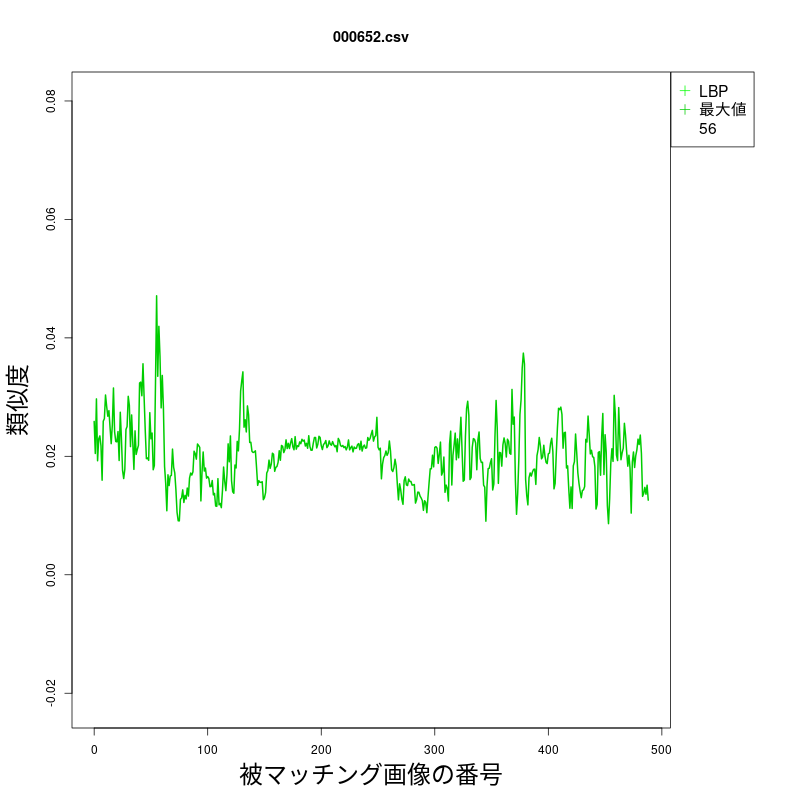
\includegraphics[pagebox=cropbox, scale=0.25]{sotuken_png/resultLBP_000652.png}
    \end{minipage}
    &
    \begin{minipage}[b]{0.5\linewidth}
      \centering
      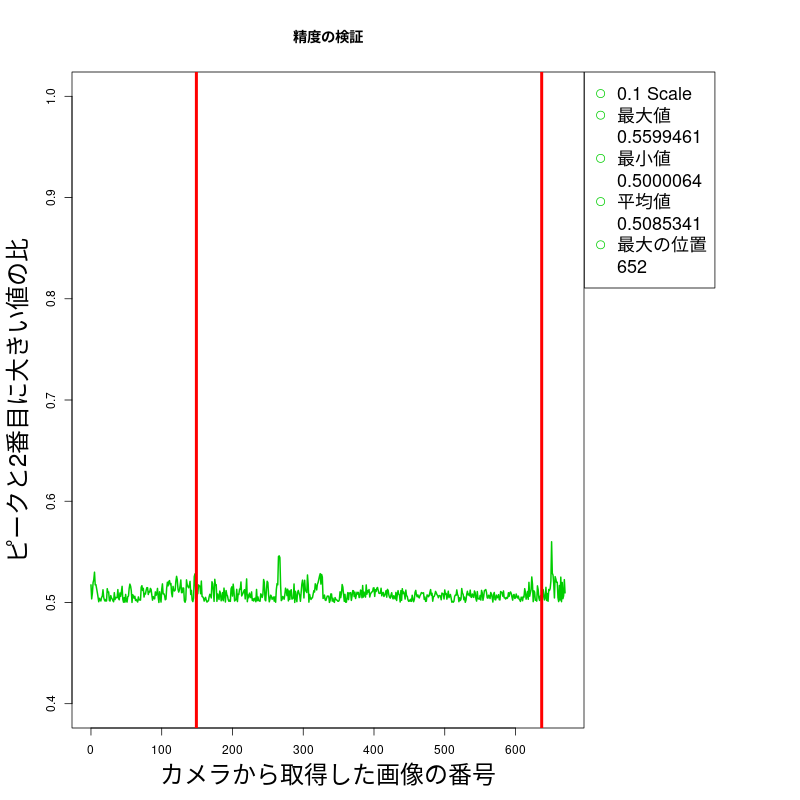
\includegraphics[pagebox=cropbox, scale=0.25]{sotuken_png/peak/peak_LBP.png}
    \end{minipage}
  \end{tabular}
  \caption{LBP特徴のみを適用時の自己位置推定の結果と精度検証}
  \label{LBPR}
\end{figure}

\begin{figure}[H]
  \centering
  \begin{tabular}{cc}
    \begin{minipage}[b]{0.5\linewidth}
      \centering
      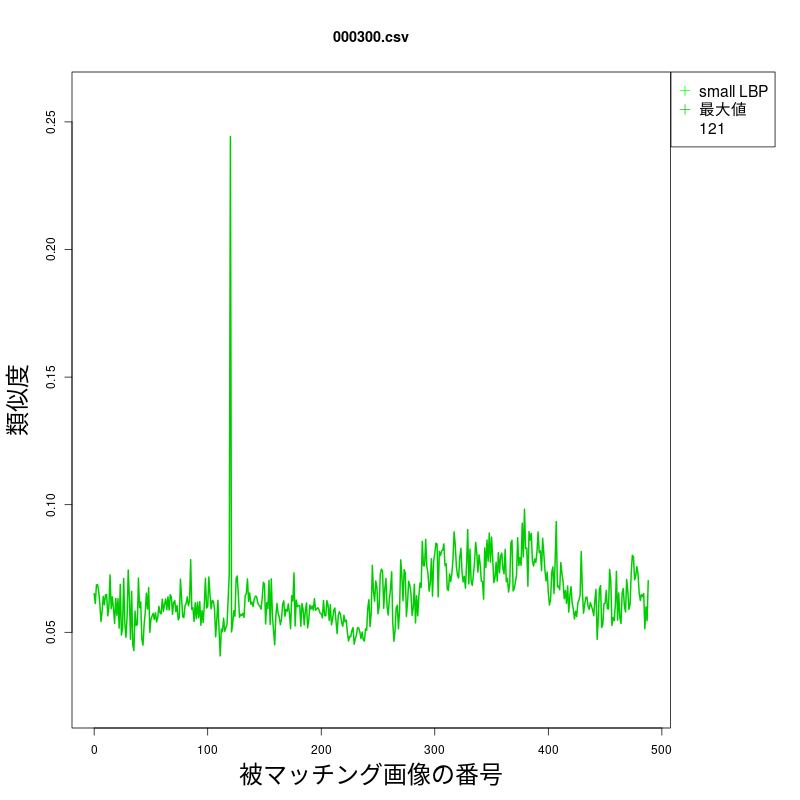
\includegraphics[pagebox=cropbox, scale=0.25]{sotuken_png/resultSLBP_000300.png}
    \end{minipage}
    &
    \begin{minipage}[b]{0.5\linewidth}
      \centering
      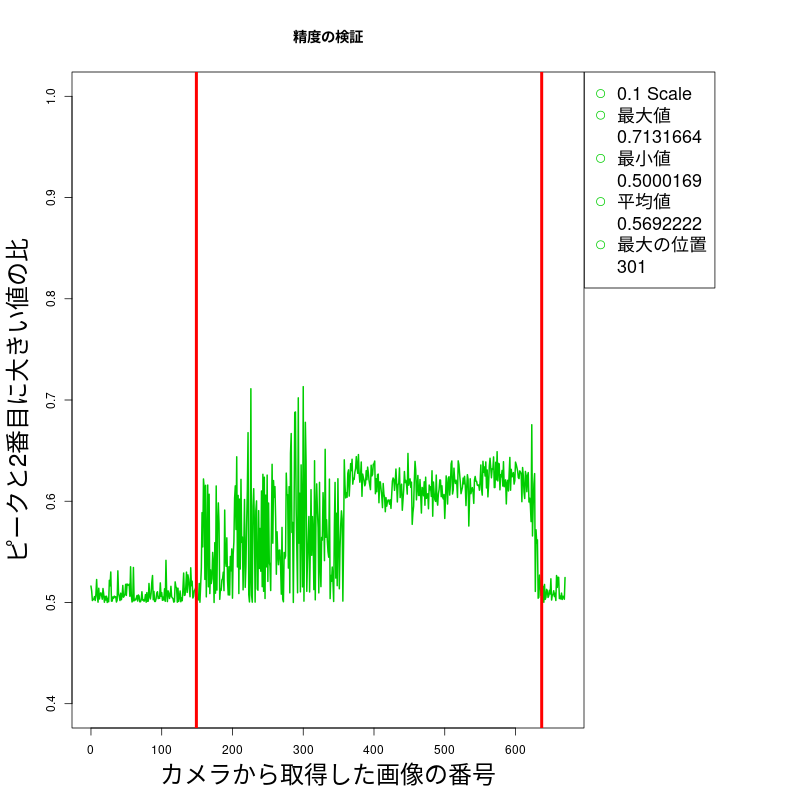
\includegraphics[pagebox=cropbox, scale=0.25]{sotuken_png/peak/peak_LBP_small.png}
    \end{minipage}
  \end{tabular}
  \caption{画像縮小とLBP特徴を適用時の自己位置推定の結果と精度検証}
  \label{SLBPR}
\end{figure}

\begin{figure}[H]
  \centering
  \begin{tabular}{cc}
    \begin{minipage}[b]{0.5\linewidth}
      \centering
      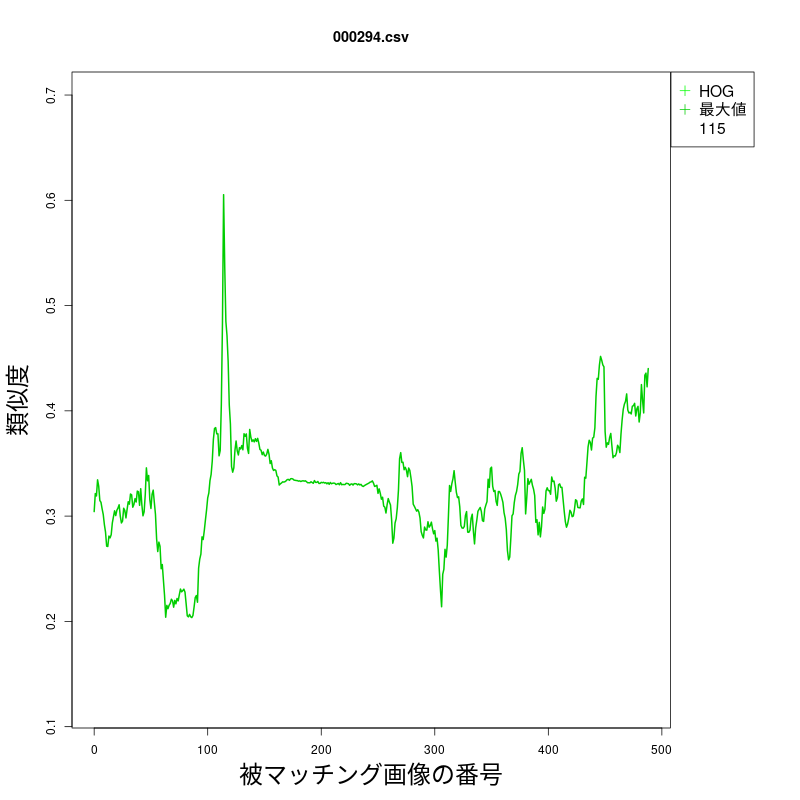
\includegraphics[pagebox=cropbox, scale=0.25]{sotuken_png/resutlHOG_000294.png}
    \end{minipage}
    &
    \begin{minipage}[b]{0.5\linewidth}
      \centering
      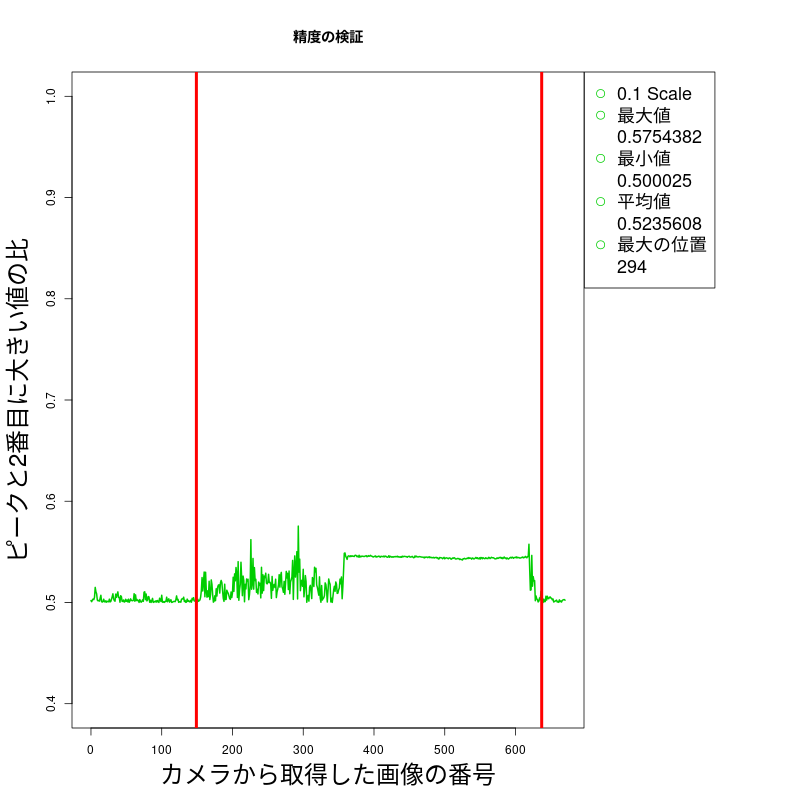
\includegraphics[pagebox=cropbox, scale=0.25]{sotuken_png/peak/peak_HOG.png}
    \end{minipage}
  \end{tabular}
  \caption{HOG特徴のみを適用時の自己位置推定の結果と精度検証}
  \label{HOGR}
\end{figure}

\begin{table}[t]
  \centering
  \caption{accuracyの最大最小と平均値のまとめ}
  \label{t1}
  \begin{tabular}{lccc}
    自己位置推定の手法&最大値&最小値&平均値\\\hline
    画像縮小&0.524&0.500&0.509\\
    Canny&0.766&0.500&0.570\\
    画像縮小+Canny&0.660&0.500&0.525\\
    LBP&0.56&0.500&0.509\\
    画像縮小+LBP&0.713&0.500&0.569\\
    HOG&0.575&0.500&0.523\\
  \end{tabular}
\end{table}
図\ref{tempR}から図\ref{HOGR}の左の画像はそれぞれの画像特徴を使用した時の自己位置推定の結果の中でも
最も顕著なピークが得られた結果となっている。また、左の画像が精度検証によって得られたグラフとなっている。

実験の結果のグラフの中で最もピークがたっている部分がカメラから取得した風景画像と事前走行画像を照合した結果
最も類似度が高いと識別された所である。
そのため、ピークのところが現在地とみなされている風景画像である。

画像縮小のみとLBP特徴のみ以外の4種類の画像特徴で顕著なピークを得られていることが図\ref{tempR}から図\ref{HOGR}の左のグラフから分かる
自己位置推定の結果のグラフの中で顕著なピークが得られている画像特徴は精度検証のグラフの中でも高い精度を得ることができている。

表\ref{t1}はそれぞれの画像特徴に対して行った精度検証の中の最大値、最小値、平均値をまとめたものである。
表\ref{t1}を見ると精度が最も高い値を持っている画像特徴はCannyのエッジ検出のみを使用した時である。
次点で画像縮小してLBP特徴を使用した時となっている。平均値も同様の順になっている。
平均値について、精度検証の最大値が近い値ではないのに画像縮小してCannyのエッジ検出とHOG特徴のみを使用した時が近い値を持つことがわかった。

\section{考察}
実験結果から画像特徴ごとの自己位置推定の類似度のグラフに特徴が出ていることが分かった。
ピークが顕著に現れている画像特徴はCannyのエッジ検出を使用した時、画像縮小とCannyのエッジ検出をを照合した時、
画像縮小とLBP特徴を使用した時とHOG特徴のみを使用した時である。
それぞれの画像特徴でなぜピークが顕著に現れた理由を考えていくと
Cannyのエッジ検出を行う事で図\ref{CANimg}のような建物や山並みなどの輪郭線のみの画像となっており、
輪郭線が一致した時と一致していない時では照合時の結果に差が出るのだと予想することができる。
画像縮小とLBP特徴を使用した時では、画像縮小によって画像内に写る建物などの大まかな形状を取り出すことができ、
LBP特徴による天候の変化による照明の影響を受けにくくするする特徴が上手く働いたのだと予想することができる。
HOG特徴のみを使用した時では、画像内の建物や看板などの形状をより強調することができており、
形状の特徴と元の風景の二つの情報で照合を行っているため、一致している部分でピークが高くなっているのだと予想することができる。

次に精度検証によって得られた結果についてみていく。
まず、精度検証の結果のグラフに描かれている2本の赤い縦線については、縦線と縦線の間の区間が
今回使用した群馬大学周りの青い経路と赤い経路の同一区間であることを表している。
表\ref{t1}より、accuracyの最大値が0.6を超えている画像特徴がCannyのエッジ検出のみ、画像縮小してCannyのエッジ検出と画像縮小してLBP特徴の3つである。
その中でも、Cannyのエッジ検出のみと画像縮小してLBP特徴を使用した時のグラフは似ており、
画像縮小してCannyのエッジ検出をしたときとは違うグラフとなっている。
これは、同一区間の後半の部分では青い経路の画像軍は信号の前で停車している時の風景画像が映し出されているが、
この時の画像照合ができているかどうかの差であると見られる。
図\ref{400F}は青い経路の画像群で赤信号で停車中の時の自己位置推定の結果である。
これを見るとCannyのエッジ検出のみの時と画像縮小してLBP特徴の時にはピークが立っているが、
画像縮小してCannyのエッジ検出をした時ではピークが乱立していることがわかる。
実際にCannyのエッジ検出で画像縮小しない場合とした場合の画像照合で使用された画像を確認すると図\ref{400Fimg}となっている。
図\ref{400Fimg}を見ると画像縮小した場合としなかった場合では検出できた輪郭線の密度に違いがみられる。
そのため、本来不一致な部分でも輪郭線の密度の差から一致とみなされてしまったのではないかと予想される。

\section{おわりに}
本研究では自動運転の基幹技術の中のひとつである自己位置推定について、その手法の一つであるシーンマッチングに着目して
人間と同じように今見ている風景を事前走行時に作成した風景画像のデータベースと照合することで現在地を推定できるかどうかを調べた。
結果としては、画像特徴を使用、組み合わせることで照合の精度を上げ、より現在地に近い地点の画像を得ることができた。
今後は実際に自動運転車両に搭載するにあたっての必要な要件満たし、さらに精度の高い自己位置推定の手法を模索していきたい。

\section{参考文献}
\begin{thebibliography}{99}
  \bibitem{f1} SUBARUの総合安全, 株式会社SUBARU, 2023-02-10 閲覧\url{https://www.subaru.jp/safety/eyesight/}
  \bibitem{f2} Tesla MODEL3, Tesla Mortors, 2023-02-10 閲覧\url{https://www.tesla.com/ja_jp/model3}
  \bibitem{f3} TOYOTA Advanced Drive 株式会社TOYOTA, 2023-02-10 閲覧 \url{https://toyota.jp/mirai/feature/?padid=from_mirai_top_topics_advanceddrive#ft-dspt}
  \bibitem{f4} Canny, J.、A Computational Approach To Edge Detection、IEEE Transactions on Pattern Analysis and Machine Intelligence, December1986 pp.679–698.
  \bibitem{f5} T. Ojala, M. Pietikainen, D. Harwood, "Performance evaluation of texture measures with classification based on Kullback discrimination of distributions", Proceedings of 12th International Conference on Pattern Recognition, Octorber 1994, vol. 1, pp. 582-586.
  \bibitem{f6} Faith Porikli,"Integral Histogram: A Fast Way to Extract Histograms in Cartesian Spaces" , IEEE Conference on Computer Vision and Pattern Recognition (CVPR), June 2005, vol. 1, pp. 829-836.
  \bibitem{f7} N. Dalal, B.B Triggs, "Histograms of oriented gradients for human detection", 2005 IEEE Computer Society Conference on Computer Vision and Pattern Recognition (CVPR'05), June 2005, vol. 1, pp. 886-893.
\end{thebibliography}
\section{付録}

\begin{figure}[H]
  \centering
  \begin{tabular}{cc}
    \begin{minipage}[b]{0.5\linewidth}
      \centering
      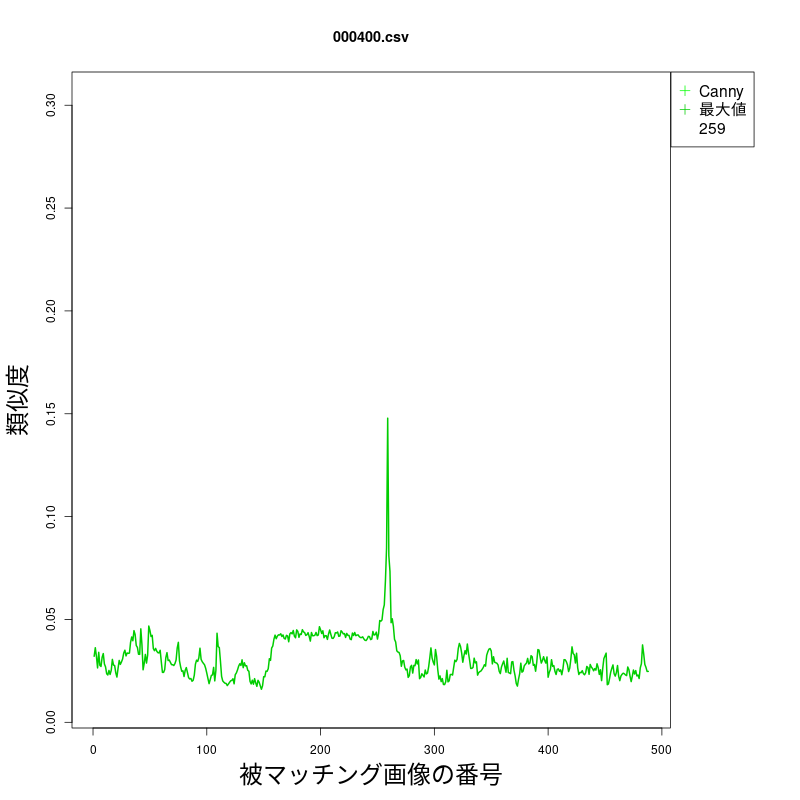
\includegraphics[pagebox=cropbox, scale=0.2]{sotuken_png/resultCanny_000400.png}
      \subcaption{Cannyのエッジ検出のみ}
    \end{minipage}
    &
    \begin{minipage}[b]{0.5\linewidth}
      \centering
      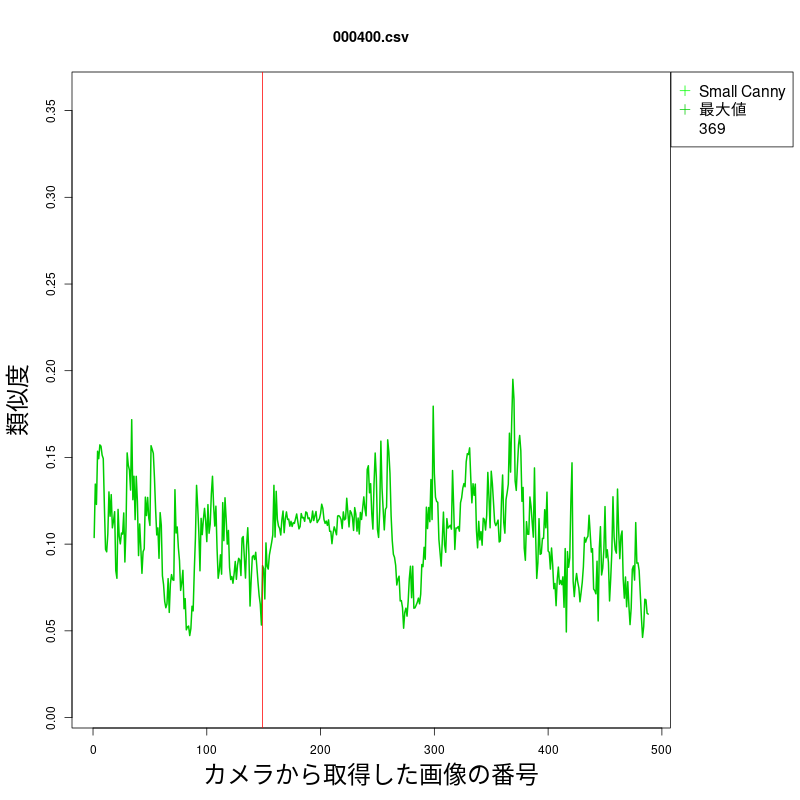
\includegraphics[pagebox=cropbox, scale=0.2]{sotuken_png/resultSCanny_000400.png}
      \subcaption{画像縮小+Cannyのエッジ検出}
    \end{minipage}
    \\
    \begin{minipage}[b]{0.5\linewidth}
      \centering
      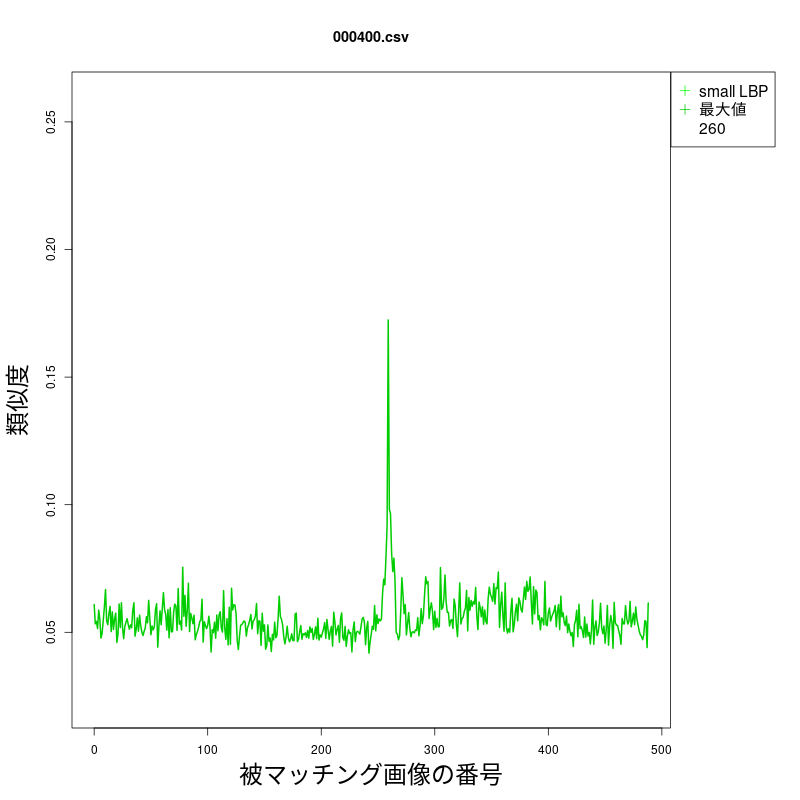
\includegraphics[pagebox=cropbox, scale=0.2]{sotuken_png/resultSLBP_000400.png}
      \subcaption{画像縮小+LBP特徴}
    \end{minipage}
    &
  \end{tabular}
  \caption{それぞれの画像特徴の400フレーム目の自己位置推定の結果}
  \label{400F}
\end{figure}

\begin{figure}[H]
  \centering
  \begin{tabular}{cc}
    \begin{minipage}[b]{0.5\linewidth}
      \centering
      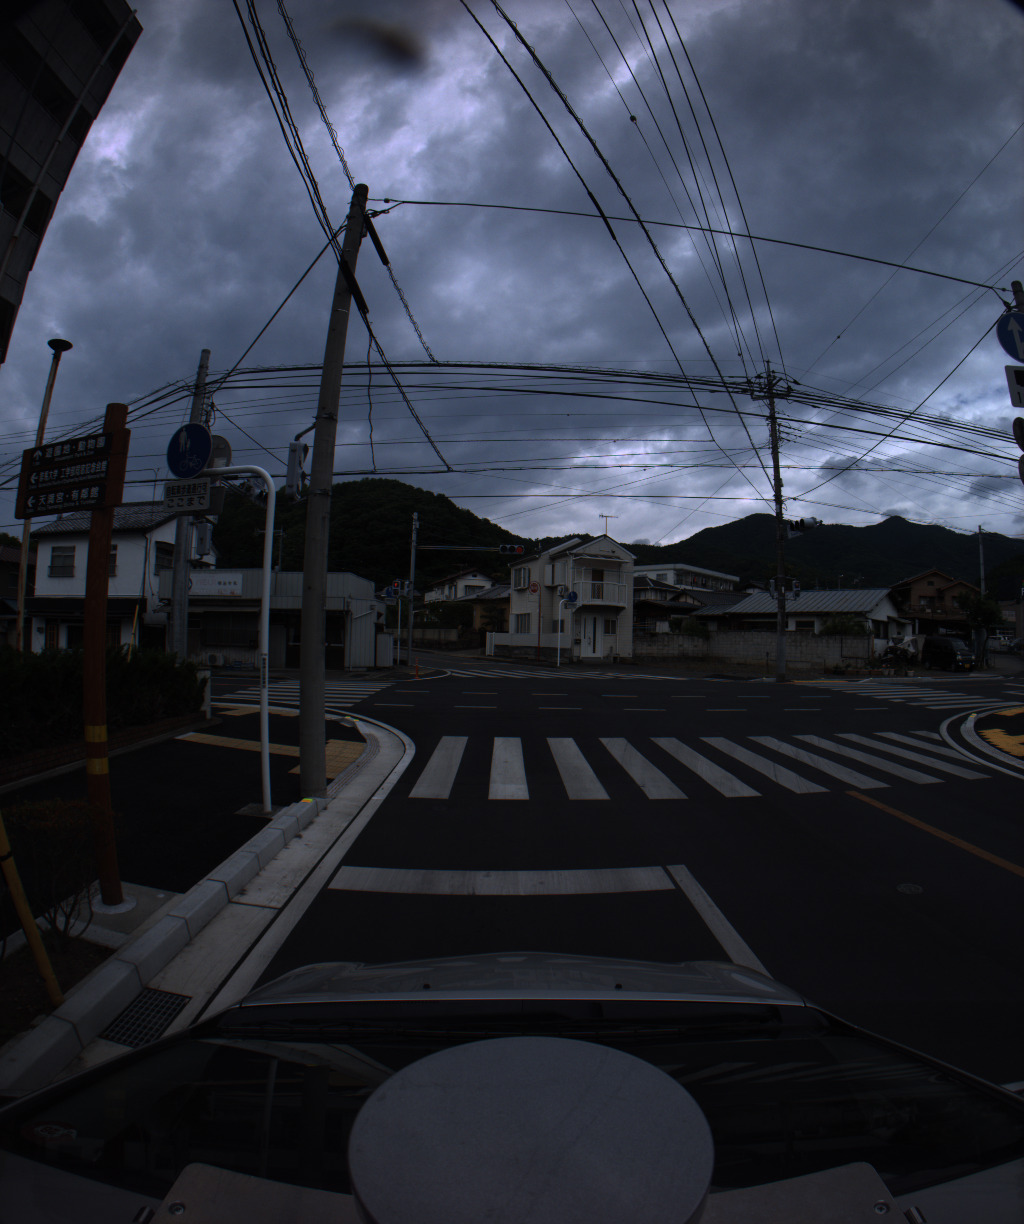
\includegraphics[pagebox=cropbox, scale=0.1]{sotuken_png/Test00_000400.jpg}
      \subcaption{曇り }
    \end{minipage}
    &
    \begin{minipage}[b]{0.5\linewidth}
      \centering
      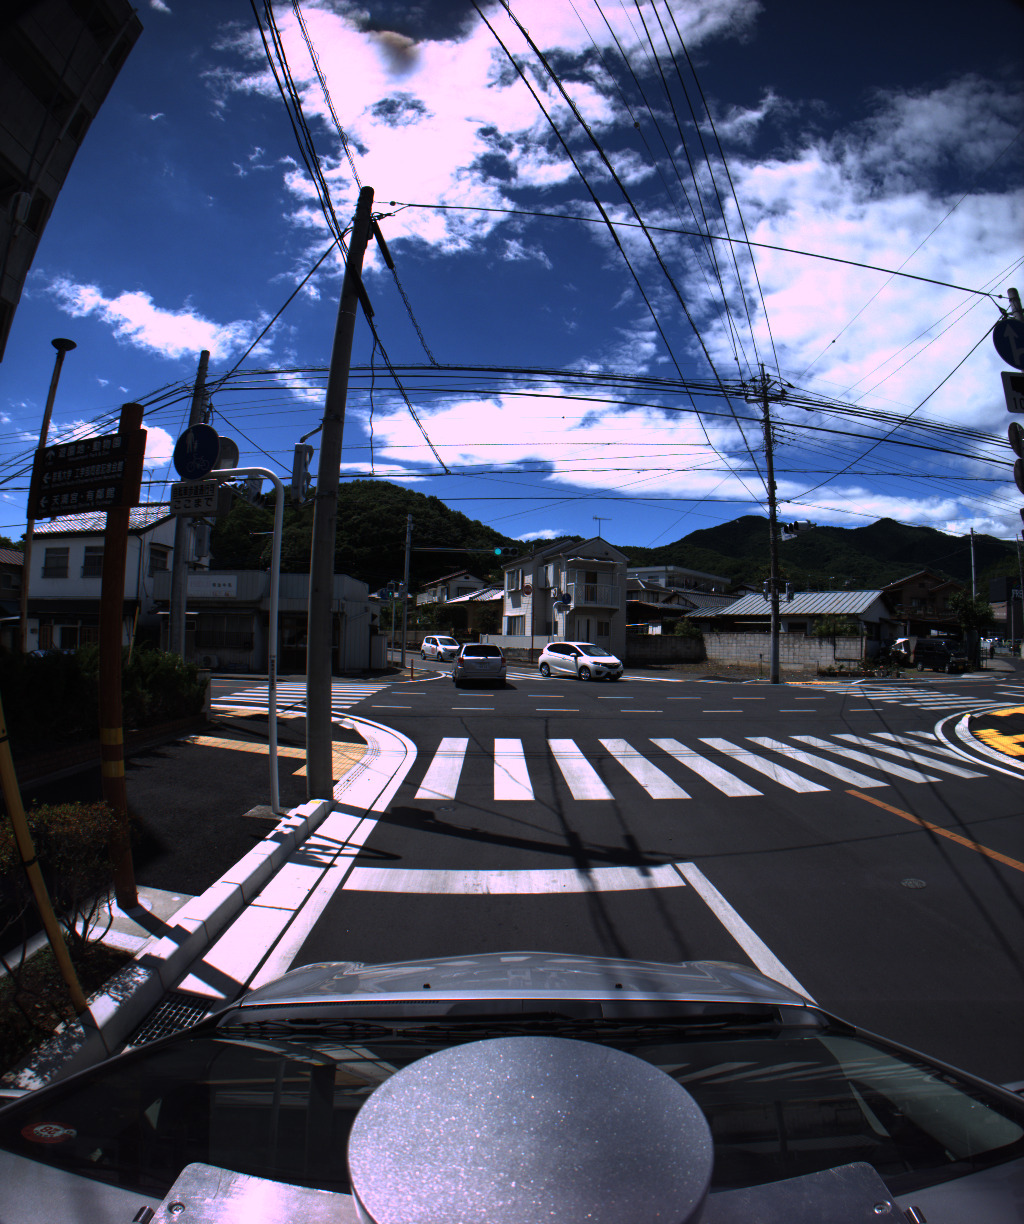
\includegraphics[pagebox=cropbox, scale=0.1]{sotuken_png/Test01_000259.jpg}
      \subcaption{晴れ}
    \end{minipage}
    \\
    \begin{minipage}[b]{0.5\linewidth}
      \centering
      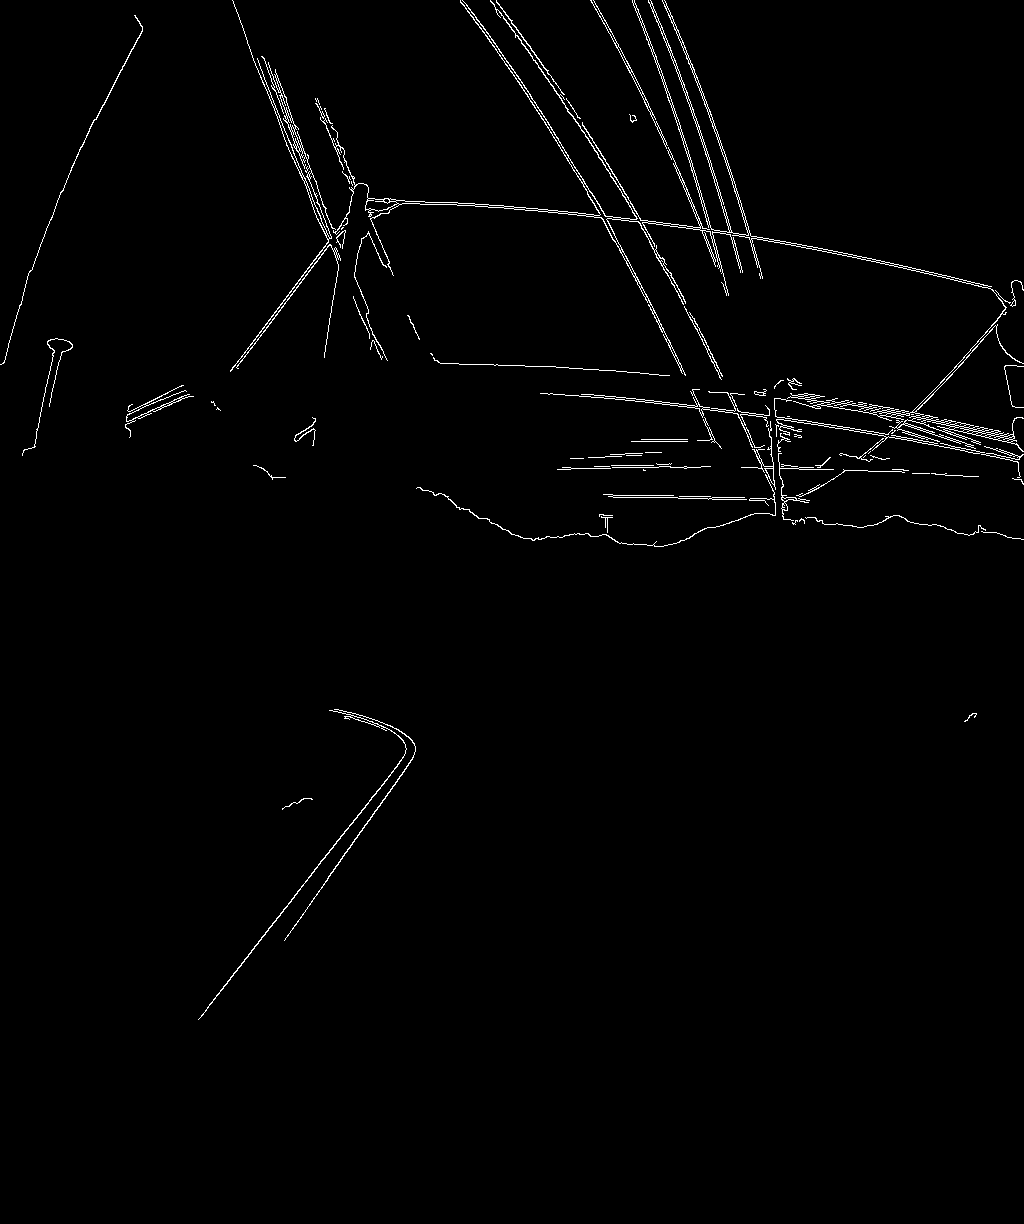
\includegraphics[pagebox=cropbox, scale=0.1]{sotuken_png/canny_400.png}
      \subcaption{曇り Cannyのエッジ検出のみ}
    \end{minipage}
    &
    \begin{minipage}[b]{0.5\linewidth}
      \centering
      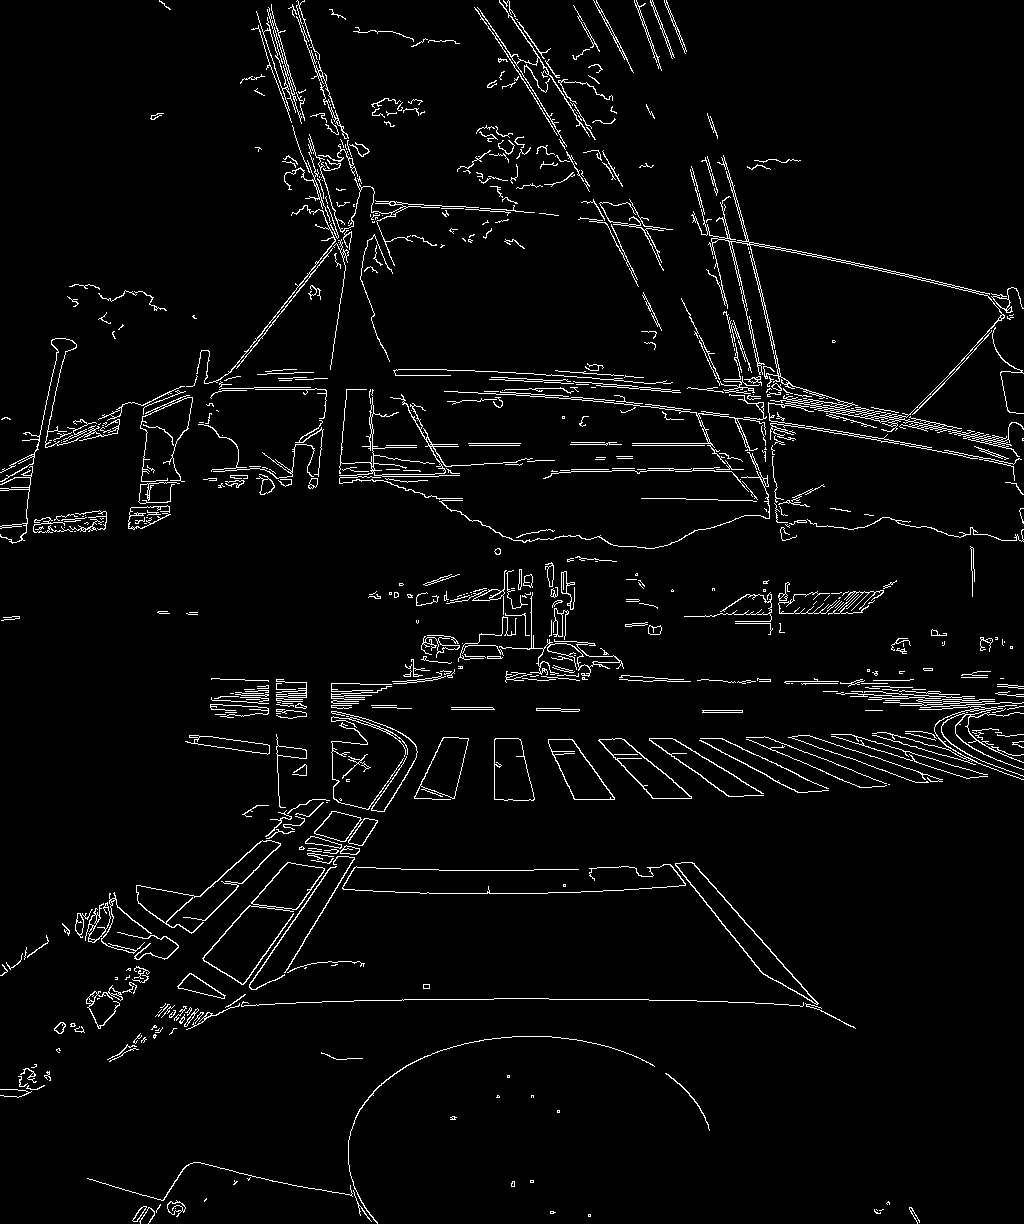
\includegraphics[pagebox=cropbox, scale=0.1]{sotuken_png/canny2_400.png}
      \subcaption{晴れ Cannyのエッジ検出のみ}
    \end{minipage}
    \\
    \begin{minipage}[b]{0.5\linewidth}
      \centering
      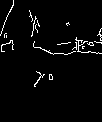
\includegraphics[pagebox=cropbox, scale=1]{sotuken_png/scanny_400.png}
      \subcaption{曇り 画像縮小+Cannyのエッジ検出}
    \end{minipage}
    &
    \begin{minipage}[b]{0.5\linewidth}
      \centering
      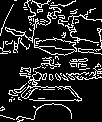
\includegraphics[pagebox=cropbox, scale=1]{sotuken_png/scanny2_400.png}
      \subcaption{晴れ 画像縮小+Cannyのエッジ検出}
    \end{minipage}

  \end{tabular}
  \caption{赤信号で停車している時の風景画像に画像特徴を適用した時の結果画像}
  \label{400Fimg}
\end{figure}

\end{document}